\documentclass[11pt,a4paper,oneside]{report}             % Single-side
%\documentclass[11pt,a4paper,twoside,openright]{report}  % Duplex

% thanks to http://tex.stackexchange.com/a/47579/71109
\usepackage{ifxetex}
\usepackage{ifluatex}
\newif\ifxetexorluatex % a new conditional starts as false
\ifnum 0\ifxetex 1\fi\ifluatex 1\fi>0
   \xetexorluatextrue
\fi

\ifxetexorluatex
  \usepackage{fontspec}
\else
  \usepackage[T1]{fontenc}
  \usepackage[utf8]{inputenc}
  \usepackage[lighttt]{lmodern}
  \ttfamily\DeclareFontShape{T1}{lmtt}{m}{it}{<->sub*lmtt/m/sl}{}
\fi

\usepackage[english,magyar]{babel} % Alapértelmezés szerint utoljára definiált nyelv lesz aktív, de később külön beállítjuk az aktív nyelvet.

\usepackage{emptypage} % omit page number on empty pages

%\usepackage{cmap}
\usepackage{amsfonts,amsmath,amssymb} % Mathematical symbols.
%\usepackage[ruled,boxed,resetcount,linesnumbered]{algorithm2e} % For pseudocodes. % beware: this is not compatible with LuaLaTeX, see http://tex.stackexchange.com/questions/34814/lualatex-and-algorithm2e
\usepackage{booktabs} % For publication quality tables for LaTeX
\usepackage{graphicx}

%\usepackage{fancyhdr}
%\usepackage{lastpage}

\usepackage{geometry}
%\usepackage{sectsty}
\usepackage{setspace} % For setting line spacing

\usepackage[unicode]{hyperref} % For hyperlinks in the generated document.
\usepackage{xcolor}
\usepackage{listings} % For source code snippets.

\usepackage[amsmath,thmmarks]{ntheorem} % Theorem-like environments.

\usepackage[hang]{caption}
\usepackage{svg}

\singlespacing

\newcommand{\selecthungarian}{
	\selectlanguage{magyar}
	\setlength{\parindent}{2em}
	\setlength{\parskip}{0em}
	\frenchspacing
}

\newcommand{\selectenglish}{
	\selectlanguage{english}
	\setlength{\parindent}{0em}
	\setlength{\parskip}{0.5em}
	\nonfrenchspacing
	\onehalfspacing
	\renewcommand{\figureautorefname}{Figure}
	\renewcommand{\tableautorefname}{Table}
	\renewcommand{\partautorefname}{Part}
	\renewcommand{\chapterautorefname}{Chapter}
	\renewcommand{\sectionautorefname}{Section}
	\renewcommand{\subsectionautorefname}{Section}
	\renewcommand{\subsubsectionautorefname}{Section}
}

\usepackage[numbers]{natbib}
\usepackage{xspace}


%TODO Set the main variables
\newcommand{\vikszerzoVezeteknev}{Buzás}
\newcommand{\vikszerzoKeresztnev}{Gergő}

\newcommand{\vikkonzulensAMegszolitas}{Dr.~}
\newcommand{\vikkonzulensAVezeteknev}{Marussy}
\newcommand{\vikkonzulensAKeresztnev}{Kristóf}

\newcommand{\vikkonzulensBMegszolitas}{}
\newcommand{\vikkonzulensBVezeteknev}{}
\newcommand{\vikkonzulensBKeresztnev}{}

\newcommand{\vikkonzulensCMegszolitas}{}
\newcommand{\vikkonzulensCVezeteknev}{}
\newcommand{\vikkonzulensCKeresztnev}{}

\newcommand{\vikcim}{Infrastructure design and deployment of a cloud-based graph generator} % Cím
\newcommand{\viktanszek}{\bmemit} % Tanszék
\newcommand{\vikdoktipus}{\bsc} % Dokumentum típusa (\bsc vagy \msc)
\newcommand{\vikmunkatipusat}{szakdolgozatot} % a "hallgató nyilatkozat" részhez: szakdolgozatot vagy diplomatervet

\input{include/tdk-variables}
\newcommand{\szerzoMeta}{\vikszerzoVezeteknev{} \vikszerzoKeresztnev} % egy szerző esetén
%\newcommand{\szerzoMeta}{\vikszerzoVezeteknev{} \vikszerzoKeresztnev, \tdkszerzoB} % két szerző esetén

%TODO Language configuration -- choose one
% Beállítások magyar nyelvű dolgozathoz
%%--------------------------------------------------------------------------------------
% Elnevezések
%--------------------------------------------------------------------------------------
\newcommand{\bme}{Budapesti Műszaki és Gazdaságtudományi Egyetem}
\newcommand{\vik}{Villamosmérnöki és Informatikai Kar}

\newcommand{\bmemit}{Mesterséges Intelligencia és Rendszertervezés Tanszék}

\newcommand{\keszitette}{Készítette}
\newcommand{\konzulens}{Konzulens}

\newcommand{\bsc}{Szakdolgozat}
\newcommand{\msc}{Diplomaterv}
\newcommand{\tdk}{TDK dolgozat}
\newcommand{\bsconlab}{BSc Önálló laboratórium}
\newcommand{\msconlabi}{MSc Önálló laboratórium 1.}
\newcommand{\msconlabii}{MSc Önálló laboratórium 2.}

\newcommand{\pelda}{Példa}
\newcommand{\definicio}{Definíció}
\newcommand{\tetel}{Tétel}

\newcommand{\bevezetes}{Bevezetés}
\newcommand{\koszonetnyilvanitas}{Köszönetnyilvánítás}
\newcommand{\fuggelek}{Függelék}

% Opcionálisan átnevezhető címek
%\addto\captionsmagyar{%
%\renewcommand{\listfigurename}{Saját ábrajegyzék cím}
%\renewcommand{\listtablename}{Saját táblázatjegyzék cím}
%\renewcommand{\bibname}{Saját irodalomjegyzék név}
%}

\newcommand{\szerzo}{\vikszerzoVezeteknev{} \vikszerzoKeresztnev}
\newcommand{\vikkonzulensA}{\vikkonzulensAMegszolitas\vikkonzulensAVezeteknev{} \vikkonzulensAKeresztnev}
\newcommand{\vikkonzulensB}{\vikkonzulensBMegszolitas\vikkonzulensBVezeteknev{} \vikkonzulensBKeresztnev}
\newcommand{\vikkonzulensC}{\vikkonzulensCMegszolitas\vikkonzulensCVezeteknev{} \vikkonzulensCKeresztnev}

\newcommand{\selectthesislanguage}{\selecthungarian}

\bibliographystyle{huplain}

\def\lstlistingname{lista}

\newcommand{\appendixnumber}{6}  % a fofejezet-szamlalo az angol ABC 6. betuje (F) lesz

% Settings for English documents
%--------------------------------------------------------------------------------------
% Elnevezések
%--------------------------------------------------------------------------------------
\newcommand{\bme}{Budapest University of Technology and Economics}
\newcommand{\vik}{Faculty of Electrical Engineering and Informatics}

\newcommand{\bmemit}{Department of Artificial Intelligence and Systems Engineering}

\newcommand{\keszitette}{Author}
\newcommand{\konzulens}{Advisor}

\newcommand{\bsc}{Bachelor's Thesis}
\newcommand{\msc}{Master's Thesis}
\newcommand{\tdk}{Scientific Students' Association Report}
\newcommand{\bsconlab}{BSc Project Laboratory}
\newcommand{\msconlabi}{MSc Project Laboratory 1}
\newcommand{\msconlabii}{MSc Project Laboratory 2}

\newcommand{\pelda}{Example}
\newcommand{\definicio}{Definition}
\newcommand{\tetel}{Theorem}

\newcommand{\bevezetes}{Introduction}
\newcommand{\koszonetnyilvanitas}{Acknowledgements}
\newcommand{\fuggelek}{Appendix}

% Optional custom titles
%\addto\captionsenglish{%
%\renewcommand*{\listfigurename}{Your list of figures title}
%\renewcommand*{\listtablename}{Your list of tables title}
%\renewcommand*{\bibname}{Your bibliography title}
%}

\newcommand{\szerzo}{\vikszerzoKeresztnev{} \vikszerzoVezeteknev}
\newcommand{\vikkonzulensA}{\vikkonzulensAMegszolitas\vikkonzulensAKeresztnev{} \vikkonzulensAVezeteknev}
\newcommand{\vikkonzulensB}{\vikkonzulensBMegszolitas\vikkonzulensBKeresztnev{} \vikkonzulensBVezeteknev}
\newcommand{\vikkonzulensC}{\vikkonzulensCMegszolitas\vikkonzulensCKeresztnev{} \vikkonzulensCVezeteknev}

\newcommand{\selectthesislanguage}{\selectenglish}

\bibliographystyle{plainnat}

\newcommand{\ie}{i.e.\@\xspace}
\newcommand{\Ie}{I.e.\@\xspace}
\newcommand{\eg}{e.g.\@\xspace}
\newcommand{\Eg}{E.g.\@\xspace}
\newcommand{\etal}{et al.\@\xspace}
\newcommand{\etc}{etc.\@\xspace}
\newcommand{\vs}{vs.\@\xspace}
\newcommand{\viz}{viz.\@\xspace} % videlicet
\newcommand{\cf}{cf.\@\xspace} % confer
\newcommand{\Cf}{Cf.\@\xspace}
\newcommand{\wrt}{w.r.t.\@\xspace} % with respect to
\newcommand{\approximately}{approx.\@\xspace}

\newcommand{\appendixnumber}{1}  % a fofejezet-szamlalo az angol ABC 1. betuje (A) lesz


\input{include/preamble}

%--------------------------------------------------------------------------------------
% Table of contents and the main text
%--------------------------------------------------------------------------------------
\begin{document}

\pagenumbering{gobble}

%TODO These includes define guidelines -- remove these
%~~~~~~~~~~~~~~~~~~~~~~~~~~~~~~~~~~~~~~~~~~~~~~~~~~~~~~~~~~~~~~~~~~~~~~~~~~~~~~~~~~~~~~
%e\include{include/guideline}
%\include{include/project}

\selectthesislanguage

%TODO Titlepage -- choose one from below
%~~~~~~~~~~~~~~~~~~~~~~~~~~~~~~~~~~~~~~~~~~~~~~~~~~~~~~~~~~~~~~~~~~~~~~~~~~~~~~~~~~~~~~
\include{include/titlepage}		   % Szakdolgozat/Diplomaterv címlap
%\include{include/titlepage-tdk}	% TDK címlap
%\include{include/titlepage-otdk}   % OTDK címlap


% Table of Contents
%~~~~~~~~~~~~~~~~~~~~~~~~~~~~~~~~~~~~~~~~~~~~~~~~~~~~~~~~~~~~~~~~~~~~~~~~~~~~~~~~~~~~~~
\tableofcontents\cleardoublepage


% Declaration and Abstract
%~~~~~~~~~~~~~~~~~~~~~~~~~~~~~~~~~~~~~~~~~~~~~~~~~~~~~~~~~~~~~~~~~~~~~~~~~~~~~~~~~~~~~~
\include{include/declaration} %TODO Hallgatói nyilatkozat -- TDK és OTDK esetén törlendő!
\pagenumbering{roman}
\setcounter{page}{1}

\selecthungarian

%----------------------------------------------------------------------------
% Abstract in Hungarian
%----------------------------------------------------------------------------
\chapter*{Kivonat}\addcontentsline{toc}{chapter}{Kivonat}

Jelen dokumentum egy diplomaterv sablon, amely formai keretet ad a BME Villamosmérnöki és Informatikai Karán végző hallgatók által elkészítendő szakdolgozatnak és diplomatervnek. A sablon használata opcionális. Ez a sablon \LaTeX~alapú, a \emph{TeXLive} \TeX-implementációval és a PDF-\LaTeX~fordítóval működőképes.



\vfill
\selectenglish


%----------------------------------------------------------------------------
% Abstract in English
%----------------------------------------------------------------------------
\chapter*{Abstract}\addcontentsline{toc}{chapter}{Abstract}

This document is a \LaTeX-based skeleton for BSc/MSc~theses of students at the Electrical Engineering and Informatics Faculty, Budapest University of Technology and Economics. The usage of this skeleton is optional. It has been tested with the \emph{TeXLive} \TeX~implementation, and it requires the PDF-\LaTeX~compiler.


\vfill
\cleardoublepage

\selectthesislanguage

\newcounter{romanPage}
\setcounter{romanPage}{\value{page}}
\stepcounter{romanPage}    %TODO Összefoglaló -- TDK és OTDK esetén nem kötelező


% The main part of the thesis
%~~~~~~~~~~~~~~~~~~~~~~~~~~~~~~~~~~~~~~~~~~~~~~~~~~~~~~~~~~~~~~~~~~~~~~~~~~~~~~~~~~~~~~
\pagenumbering{arabic}

%TODO import your own content
%----------------------------------------------------------------------------
\chapter{\bevezetes}
%----------------------------------------------------------------------------

Graph analysis problems can be approached through partial modeling. By leveraging
formal methods of partial modeling, these problems can be verified using automatically
generated test data derived from the partial model definitions.

Refinery \cite{refinery} is a cloud-based `Graph Solver as a Service' web application. It supports problem
definition for problems which can be mathematically retrieved to a graph-related problems.
The application has an editor, which constantly checks for the correctness of our problem definition:
both semantically and syntactically. The editor uses the custom-made partial modeling language of Refinery.

Users of the application can generate a model, representing their defined graph problems. The generation of 
said model can be quite resource heavy and may take several seconds to perform. 
This generation is currently performed in the same backend server, towards which the frontend clients of the application
connect and communicate with. 

Under increased usage from the users, new connections made to the backend server might not be possible because of 
the increased workloads on the server. Furthermore, response times might make the user experience worse for the users, due to the increased response
times or timeouts.

This issue should only arise, under extreme usage-circumstances. The deployed infrastructure in production already mitigates this issue by 
the use of auto scaling and load balancers. However, the model generation is still done on the same server as the backend server of 
the application.

The scope of my thesis is the designing and implementation of a generator service, which can be integrated into the workflow of the model generation.
By implementing a generator service, it is hoped, that the response times under heavy usage can improve. All of this should be performed by 
putting extra care into the scalabity of the application. The costs associated with the improvements should also be considered.

In Chapter \ref{Background}, I introduce the technologies, that are already or could be used for the 
implementation of the Refinery web application.
This is done with extra attention put towards the model generation part of the application.

In Chapter \ref{overview}, I go over the current implementation of the application. I describe the frontend and the current backend of the application.
At the end, I set requirements for the modification of the application, which should be considered for all of the latter parts of the thesis.

In Chapter \ref{considerations}, I list the possible implementations for the generator service. The advantages and disadvantages of all implementation 
possibilities are considered both architecturally and infrastructurally. I compare the possibilities and draw a conclusion, of what should be implemented.

In Chapter \ref{Implementation}, I implement the architectural and the infrastructural changes that were designed in Chapter \ref{considerations}.

In Chapter \ref{Evaluation}, I evaluate how the changes implemented in chapter \ref{Implementation} satisfy the requirements made 
in section \ref{requirements}. I benchmark the new implementation compared to the old implementation. I draw a conclusion, how succesful the 
project was.

Last, but not least, in Chapter \ref{Conclusion}, I summarize the results and desribe the future improvements that can or need to be 
done in the future.

\chapter{Background} \label{Background}
\section{Refinery}
	Refinery \cite{refinery} is an open-source framework designed to automate the synthesis of diverse, consistent domain-specific graph models. 
	It features a high-level specification language that leverages partial models to concisely define a variety of graph generation challenges. 
	With its modern, cloud-based architecture, Refinery provides a scalable "Graph Solver as a Service" that applies logic-based reasoning rules to 
	efficiently produce diverse solutions by refining partial models. This framework supports applications such as system-level architecture synthesis,
	test generation for modeling tools, and traffic scenario synthesis for autonomous vehicles.

	Refinery is also hosted as a web application at "https://refinery.services" and can be used as a standalone service.
	This application allows the user to define their graph modelling problems using the specification language. 

\section{Java}
	Java \cite{java} is a widely-used, object-oriented programming language known for its platform independence, achieved through the Java Virtual Machine (JVM) 
	which allows Java applications to run on any device or operating system. This portability, combined with its robustness, scalability, and extensive libraries,
	makes Java a popular choice for developing enterprise-level applications, web services, and backend systems.

	Java supports core object-oriented programming principles like encapsulation, inheritance, and polymorphism, promoting code modularity and reusability.
	Additionally, Java’s memory management is handled through an automatic garbage collector, which improves performance by reclaiming memory used by objects 
	that are no longer accessible. The garbage collector (GC) also helps developers, so that they don't have to think about memory management when writing code in Java.
	With lower lever languages like C and C++, memory management has been a constant issue, as memory leakages worsen performance and software security can be hurt.
	Java also has a strong emphasis on security, providing a secure runtime environment through features such as bytecode 
	verification and sandboxing, which helps prevent unauthorized access and code manipulation.

	When working with Java, a Java Development Kit (JDK) has to be installed on the system.
	The Java Development Kit (JDK) is a distribution of Java technology by Oracle Corporation. 
	It implements the Java Language Specification (JLS) and the Java Virtual Machine Specification (JVMS) 
	and provides the Standard Edition (SE) of the Java Application Programming Interface (API). 

\section{Gradle}
	Gradle \cite{gradle} is a build automation tool for multi-language software development. It controls the development process in the tasks of compilation 
	and packaging to testing, deployment, and publishing. Supported languages include Java (as well as Kotlin, Groovy, Scala), C/C++, and JavaScript.
	Gradle builds on the concepts of Apache Ant and Apache Maven, and introduces a Groovy- and Kotlin-based domain-specific language contrasted with 
	the XML-based project configuration used by Maven. Gradle uses a directed acyclic graph to determine the order in which tasks can be run, 
	through providing dependency management. It runs on the Java Virtual Machine.

	Gradle was designed for multi-project builds, which can grow to be large. It operates based on a series of build tasks that can run serially or in parallel.
	Incremental builds are supported by determining the parts of the build tree that are already up to date; any task dependent only on those parts does not need 
	to be re-executed. It also supports caching of build components, potentially across a shared network using the Gradle Build Cache. 
	The software is extensible for new features and programming languages with a plugin subsystem. 

\section{Jetty}
	Eclipse Jetty \cite{jetty} provides a highly scalable and memory-efficient web server and servlet container, supporting many protocols
	 such as HTTP/3,2,1 and WebSocket.

\section{JSON}
	JSON (JavaScript Object Notation) \cite{json} is a lightweight data-interchange format. It is easy for humans to read and write. 
	It is easy for machines to parse and generate. It is based on a subset of the JavaScript Programming Language Standard ECMA-262 3rd Edition - December 1999.
	JSON is a text format that is completely language independent but uses conventions 
	that are familiar to programmers of the C-family of languages, including C, C++, \text{C\#}, Java, JavaScript, Perl, Python, and many others. These properties make JSON an ideal data-interchange language.

	JSON is built on two structures:

	\begin{itemize}
		\item A collection of name/value pairs. In various languages, this is realized as an object, record, struct, dictionary, hash table, 
		keyed list, or associative array.
		\item An ordered list of values. In most languages, this is realized as an array, vector, list, or sequence.
	\end{itemize}

	These are universal data structures. Virtually all modern programming languages support them in one form or another. 
	It makes sense that a data format that is interchangeable with programming languages also be based on these structures.

	In JSON, they take on these forms:

	\begin{itemize}
		\item An object is an unordered set of name/value pairs.
		\item An object begins with left brace and ends with right brace.
		\item Each name is followed by colon and the name/value pairs are separated by comma.
	\end{itemize}

\section{REST API}
	A REST API \cite{restapi} (also called a RESTful API or RESTful web API) is an application programming interface (API) that conforms to the design principles of 
	the representational state transfer (REST) architectural style. REST APIs provide a flexible, lightweight way to integrate applications and to connect 
	components in microservices architectures.

	REST APIs communicate through HTTP requests to perform standard database functions like creating, reading,
	updating and deleting records (also known as CRUD operations) within a resource.

	REST API would use a GET request to retrieve a record. A POST request creates a new record. A PUT request updates a record, and a DELETE request deletes one. 
	All HTTP methods can be used in API calls. A well-designed REST API is similar to a website running in a web browser with built-in HTTP functionality.

\section{Remote Procedure Call}
	In distributed computing, a remote procedure call (RPC) \cite{rpc} is when a computer program causes a procedure (subroutine) to execute in a different address space 
	(commonly on another computer on a shared computer network), which is written as if it were a normal (local) procedure call, without the programmer 
	explicitly writing the details for the remote interaction. That is, the programmer writes essentially the same code whether the subroutine is local to 
	the executing program, or remote.
	This is a form of client–server interaction (caller is client, executor is server), typically implemented via a request–response message passing system.

\section{gRPC}
	gRPC (gRPC Remote Procedure Calls) \cite{grpcwiki} is a cross-platform high-performance remote procedure call (RPC) framework. 
	gRPC was initially created by Google, but is open source and is used in many organizations. 
	Use cases range from microservices to the "last mile" of computing (mobile, web, and Internet of Things). 
	gRPC uses HTTP/2 for transport, Protocol Buffers as the interface description language, and provides features such as authentication,
	bidirectional streaming and flow control, blocking or nonblocking bindings, and cancellation and timeouts. 
	It generates cross-platform client and server bindings for many languages. Most common usage scenarios include connecting services in a microservices 
	style architecture, or connecting mobile device clients to backend services.

	In gRPC, a client application can directly call a method on a server application on a different machine as if it were a local object, 
	making it easier for you to create distributed applications and services. As in many RPC systems, gRPC is based around the idea of 
	defining a service, specifying the methods that can be called remotely with their parameters and return types. \cite{grpcspec}
	
	\begin{figure}[h!]
		\begin{center}
			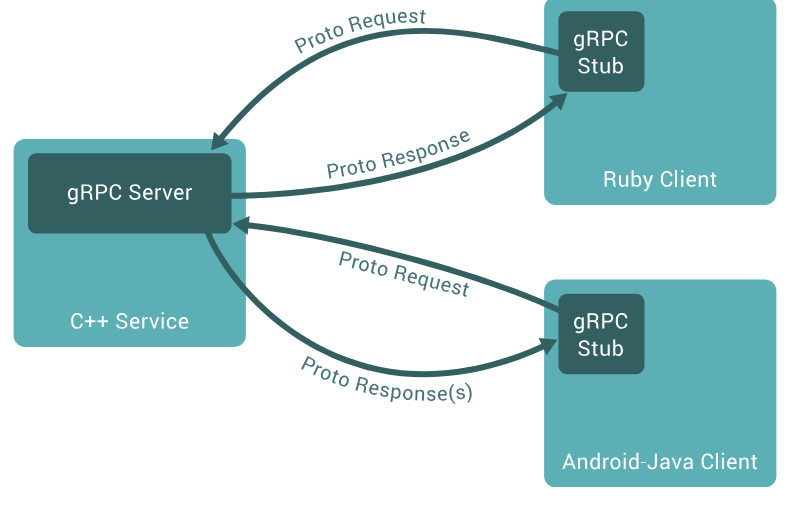
\includegraphics[scale=0.8]{include/imgs/grpc_works.PNG}	
		\end{center}
		\caption{gRPC server and the clients \cite{grpcspec}}
	\end{figure}

	On the server side, the server implements this interface and runs a gRPC server to handle client calls. On the client side, the
	client has a stub (referred to as just a client in some languages) that provides the same methods as the server.

	gRPC clients and servers can run and talk to each other in a variety of environments - from servers inside Google to your own desktop - 
	and can be written in any of gRPC’s supported languages. So, for example, you can easily create a gRPC server in Java with clients 
	in Go, Python, or Ruby. In addition, the latest Google APIs will have gRPC versions of their interfaces, letting you easily build Google functionality 
	into your applications.

	\subsection{Core concepts}

	Some of the core concepts of gRPC include \cite{grpcspec2}:
	\begin{itemize}
		\item \textbf{Unary RPC:} This is the simplest type of RPC. The client sends a single message and receives a single response. 
		\item \textbf{Server streaming RPC:} The server responds with multiple responses to the client. 
		After sending all its messages, the server’s status details (status code and optional status message) and optional trailing metadata are sent to the client.
		This completes processing on the server side. The client completes once it has all the server’s messages.
		\item \textbf{Client streaming RPC:} The client sends multiple messages and the server responds with one response message (along with its status details and optional trailing metadata). 
		\item \textbf{Bidirectional streaming RPC:} The call is initiated by the client invoking the method and the server receiving the client metadata, method name, and deadline. The server can choose to send back its initial metadata or wait for the client to start streaming messages.
		Client- and server-side stream processing is application specific. Since the two streams are independent, the client and server can read and write messages in any order.
		\item \textbf{Deadlines/Timeouts:} gRPC allows clients to specify how long they are willing to wait for an RPC to complete. On the server side, the server can query to see if a particular RPC has timed out, or how much time is left to complete the RPC.
		\item \textbf{RPC termination:} In gRPC, both the client and server make independent and local determinations of the success of the call, and their conclusions may not match. This means that, for example, you could have an RPC that finishes successfully on the server side (“I have sent all my responses!”) but fails on the client side (“The responses arrived after my deadline!”). It’s also possible for a server to decide to complete before a client has sent all its requests.
		\item \textbf{Cancelling an RPC:} Either the client or the server can cancel an RPC at any time. A cancellation terminates the RPC immediately so that no further work is done. The changes made before the cancellation are not rolled back.
	\end{itemize}

\section{WebSocket}
	The WebSocket Protocol \cite{websocket} enables two-way communication between a client
	running untrusted code in a controlled environment to a remote host
	that has opted-in to communications from that code.  The security
	model used for this is the origin-based security model commonly used
	by web browsers.  The protocol consists of an opening handshake
	followed by basic message framing, layered over TCP.  The goal of
	this technology is to provide a mechanism for applications that need two-way communication with servers that does
	not rely on opening multiple HTTP connections.

	\begin{figure}[h!]
		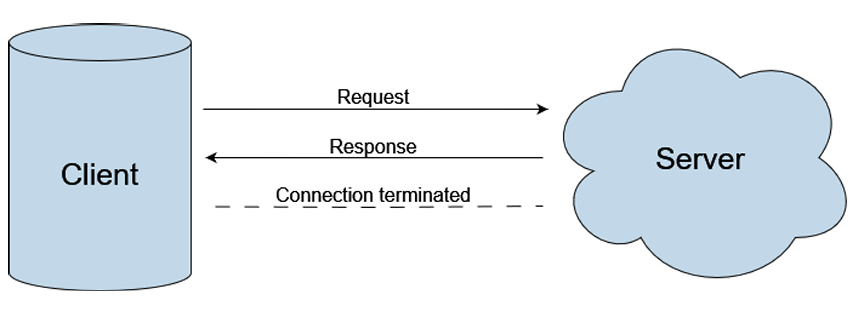
\includegraphics{include/imgs/http.PNG}
		\caption{HTTP connection}
	\end{figure}

	Historically, creating web applications that need bidirectional
	communication between a client and a server (e.g., instant messaging
	and gaming applications) has required an abuse of HTTP to poll the
	server for updates while sending upstream notifications as distinct
	HTTP calls.
	This results in a variety of problems:

	\begin{enumerate}
		\item The server is forced to use a number of different underlying TCP
		connections for each client: one for sending information to the
		client and a new one for each incoming message.
		\item The wire protocol has a high overhead, with each client-to-server
		message having an HTTP header.
		\item The client-side script is forced to maintain a mapping from the
		outgoing connections to the incoming connection to track replies.
	\end{enumerate}

	A simpler solution would be to use a single TCP connection for
	traffic in both directions.  This is what the WebSocket Protocol
	provides.

	\begin{figure}[h!]
		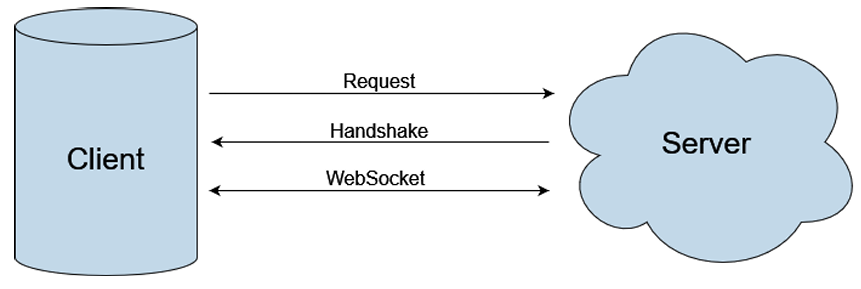
\includegraphics{include/imgs/websocket.PNG}
		\caption{WebSocket connection}
	\end{figure}

	After the initial WebSocket handshake, the communication protocol is upgraded to WebSocket from HTTP.
	If no communicaiton is happening, the connection is kept alive between the two communicating endpoints via the use of ping and pong messages.
	If a ping sender endpoint doesn't receive a pong response, the connection is lost, and the endpoints are disconnected.
	Other than that, the protocol allows for full bidirectional real-time messaging to the endpoints.

		

\section{Shell}
	In computing, a shell \cite{shell} is a computer program that exposes an operating system's services to a human user or other programs. 
	In general, operating system shells use either a command-line interface (CLI) or graphical user interface (GUI), 
	depending on a computer's role and particular operation. It is named a shell because it is the outermost layer around the operating system.

	Operating systems provide various services to their users, including file management, process management (running and terminating applications), batch processing, and operating system monitoring and configuration.

	Most operating system shells are not direct interfaces to the underlying kernel, even if a shell communicates with the user via peripheral devices 
	attached to the computer directly. Shells are actually special applications that use the kernel API in just the same way as it is used by 
	other application programs. A shell manages the user–system interaction by prompting users for input, interpreting their input, and then 
	handling output from the underlying operating system. In addition to shells running on local systems, there are different ways to make remote 
	systems available to local users; such approaches are usually referred to as remote access or remote administration.

\section{Shell script}
	A shell script \cite{shellscript} is a computer program designed to be run by a Unix shell, a command-line interpreter. The various dialects of shell scripts 
	are considered to be command languages. Typical operations performed by shell scripts include file manipulation, program execution, and printing text.
	The term is also used more generally to mean the automated mode of running an operating system shell.

\section{Cloud Computing}
	Cloud computing \cite{cloud} is the on-demand availability of computing resources (such as storage and infrastructure), as services over the internet. 
	It eliminates the need for individuals and businesses to self-manage physical resources themselves, and only pay for what they use.

	Cloud computing service models are based on the concept of sharing on-demand computing resources, software, and information over the internet. 
	Companies or individuals pay to access a virtual pool of shared resources, including compute, storage, and networking services, which are located on
	remote servers that are owned and managed by service providers. 

	One of the many advantages of cloud computing is that you only pay for what you use. This allows organizations to scale faster and more efficiently 
	without the burden of having to buy and maintain their own physical data centers and servers.  
	In simpler terms, cloud computing uses a network (most often, the internet) to connect users to a cloud platform where they request and access 
	rented computing services.

	There are three different cloud computing deployment models:
	\begin{itemize}
		\item \textbf{Public clouds} are run by third-party cloud service providers. They offer compute, storage, and network resources over the internet, 
		enabling companies to access shared on-demand resources based on their unique requirements and business goals.
		The most popular public cloud providers are Amazon, Google and Microsoft.
		\item \textbf{Private clouds} (also known as "on-premises" or "on-prem") are built, managed, and owned by a single organization 
		and privately hosted in their own data centers.
		They provide greater control, security, and management of data while still 
		enabling internal users to benefit from a shared pool of compute, storage, and network resources.
		\item \textbf{Hybrid clouds} are the mixture of using both public- and private clouds within the same organization.
	\end{itemize}

	There are three main types of cloud computing services:
	\begin{itemize}
		\item \textbf{Infrastructure as a service (IaaS)} offers on-demand access to IT infrastructure services, 
		including compute, storage, networking, and virtualization. It provides the highest level of control over your IT 
		resources and most closely resembles traditional on-premises IT resources.
		\item \textbf{Platform as a service (PaaS)} offers all the hardware and software resources needed for cloud 
		application development. With PaaS, companies can focus fully on application development without 
		the burden of managing and maintaining the underlying infrastructure.
		\item \textbf{Software as a service (SaaS)} delivers a full application stack as a service, from underlying 
		infrastructure to maintenance and updates to the app software itself. A SaaS solution is often an end-user application
		, where both the service and the infrastructure is managed and maintained by the cloud service provider.
	\end{itemize}

	\subsection{Cloud Native}
		Cloud native \cite{cloudnative} is the software approach of building, deploying, and managing modern applications 
		in cloud computing environments. Modern companies want to build highly scalable, flexible, and 
		resilient applications that they can update quickly to meet customer demands. 
		To do so, they use modern tools and techniques that inherently support application
		development on cloud infrastructure. These cloud-native technologies support fast 
		and frequent changes to applications without impacting service delivery, providing
		adopters with an innovative, competitive advantage.

	\subsection{Scaling}
		Scaling \cite{scaling} in cloud computing refers to the ability to increase or decrease IT resources as
		needed to meet changing demand. Scalability is one of the hallmarks of the cloud and the primary driver 
		of its exploding popularity with businesses. Scaling allows the businesses to pay only for the resources that
		they truly need.
		\begin{itemize}
			\item \textbf{Vertical scaling:} (also referred to as “scaling up” or “scaling down”) 
			You add or subtract power to an existing cloud server upgrading memory (RAM),
			storage or processing power (CPU).
			Usually this means that the scaling has an upper limit based on the capacity of the server
			or machine being scaled; scaling beyond that often requires downtime.
			\item \textbf{Horizontal scaling:} (also referred to as "scaling in" or "scaling out"), 
			You add more resources like servers to your system to spread out the workload across machines, 
			which in turn increases performance and storage capacity. 
			Horizontal scaling is especially important for businesses with high availability services requiring 
			minimal downtime.
		\end{itemize}

	\subsection{Load Balancing}
		Load balancing \cite{loadbalancing} is the practice of distributing computational workloads between two or more computers. 
		On the Internet, load balancing is often employed to divide network traffic among several servers. 
		This reduces the strain on each server and makes the servers more efficient, speeding up performance and 
		reducing latency. Load balancing is essential for most Internet applications to function properly. 
		By dividing user requests among multiple servers, user wait time is vastly cut down. 
		This results in a better user experience.

		Load balancing is handled by a tool or application called a load balancer. A load balancer can be 
		either hardware-based or software-based. 
		\begin{itemize}
			\item \textbf{Hardware load balancers} require the installation of a 
		dedicated load balancing device.
			\item \textbf{Software-based load balancers} can run on a server, on a virtual machine, 
		or in the cloud.
		\end{itemize}
		Content delivery networks (CDN) often include load balancing features.
		When a request arrives from a user, the load balancer assigns the request to a given server, 
		and this process repeats for each request. Load balancers determine which server should handle each request 
		based on a number of different algorithms. These algorithms fall into two main categories: static and dynamic.

		\begin{itemize}
			\item \textbf{Static load balancing} algorithms distribute workloads without taking into account the current 
			state of the system. A static load balancer will not be aware of which servers are performing 
			slowly and which servers are not being used enough. 
			Instead it assigns workloads based on a predetermined plan. 
			
			Static load balancing is quick to set up,
			but can result in inefficiencies. Round robin DNS and client-side random load balancing are 
			two common forms of static load balancing.
			\item \textbf{Dynamic load balancing} algorithms take the current availability, workload, 
			and health of each server into account. 
			They can shift traffic from overburdened or poorly performing servers to underutilized servers, 
			keeping the distribution even and efficient. However, dynamic load balancing is more difficult 
			to configure. A number of different factors play into server availability: 
			the health and overall capacity of each server, the size of the tasks being distributed, and so on.

			There are several types of dynamic load balancing algorithms, including least connection, weighted least connection, resource-based, and geolocation-based load balancing.
		\end{itemize}

\section{Amazon-related cloud technologies}
	\subsection{Amazon Web Services(AWS)}
		Amazon Web Services (AWS) is the public cloud offerring by the parent company Amazon. AWS has a vast offering
		of services, which help its end-users manage the infrastructures needed to host their own applications, 
		microservices, APIs and what not.
		AWS services are delivered to customers via a network of AWS server farms located throughout the world.

		In the following sections (2.14.2 - 2.14.6), I will go into detail what some of those services are and how
		they can be beneficial for the users of those services.

	\subsection{Amazon Elastic Compute Cloud (EC2)}
		Amazon Elastic Compute Cloud (Amazon EC2) \cite{ec2} provides on-demand, scalable computing capacity in the Amazon 
		Web Services (AWS) Cloud. Using Amazon EC2 reduces hardware costs so users can develop and deploy applications faster. 
		Amazon EC2 can be used to launch as many or as few virtual servers as needed, configure security and networking, 
		and manage storage. Capacity can be added (upscale) to handle compute-heavy tasks, such as monthly or yearly processes,
		or spikes in website traffic. When usage decreases, the capacity can be reduced (downscale) again.

		An EC2 instance is a virtual server in the AWS Cloud. When an EC2 instance is launched, the instance type that the 
		user specifies determines the hardware available to the instance. Each instance type offers a different balance of 
		compute, memory, network, and storage resources. Amazon EC2 provides the following high-level features:
		\begin{itemize}
			\item \textbf{Instances:} Virtual servers.
			\item \textbf{Amazon Machine Images (AMIs):} Preconfigured templates for the instances that package the components 
			needed for the server (including the operating system and additional software).
			\item \textbf{Instance types:} Various configurations of CPU, memory, storage, networking capacity, and graphics hardware for the instances.
			\item \textbf{Amazon EBS volumes:} Persistent storage volumes for the user's data using Amazon Elastic Block Store (Amazon EBS).
			\item \textbf{Instance store volumes:} Storage volumes for temporary data that is deleted when the user 
			stops, hibernates, or terminates their instance.
			\item \textbf{Key pairs:} Secure login information for user instances. AWS stores the public key and the user stores 
			the private key in a secure place.
			\item \textbf{Security groups:} A virtual firewall that allows users to specify the protocols, ports, and 
			source IP ranges that can reach their instances, and the destination IP ranges to which their instances can connect. 
		\end{itemize}

	\subsection{Amazon Elastic Container Service (ECS)}
		Amazon Elastic Container Service (Amazon ECS) \cite{ecs} is a fully managed container orchestration service that helps 
		you easily deploy, manage, and scale containerized applications. As a fully managed service, Amazon ECS comes 
		with AWS configuration and operational best practices built-in. It's integrated with both AWS and third-party tools, 
		such as Amazon Elastic Container Registry and Docker. This integration makes it easier for teams to focus on 
		building the applications, not the environment. You can run and scale your container workloads across AWS 
		Regions in the cloud, and on-premises, without the complexity of managing a control plane.

		There are three main layers in Amazon ECS:
		\begin{enumerate}
			\item \textbf{Capacity:} The infrastructure where the users runs their containers. Options include Amazon EC2, 
			AWS Fargate (a serverless, pay-as-you-go compute engine, where the server doesn't have to be managed for our service to run),
			and On-prem virtual machines and servers (infrastructure outside of Amazon) 
			\item \textbf{Controller:} The deployment and management of the applications that are run on the containers. The Amazon
			ECS scheduler is the software that manages / controls the applications.
			\item \textbf{Provisioning:} The tools used for interfacing with the ECS scheduler to deploy and manage the applications.
			and containers. Options include the AWS Management Console (Web GUI), AWS Command Line Interface (CLI), 
			AWS Software Development Kits (SDKs).
		\end{enumerate}

	\subsection{Virtual Private Cloud (VPC)}
		With Amazon Virtual Private Cloud (Amazon VPC) \cite{vpc}, you can launch AWS resources in a logically 
		isolated virtual network that you've defined. This virtual network closely resembles a traditional network 
		that you'd operate in your own data center, with the benefits of using the scalable infrastructure of AWS.

		Features include:
		\begin{itemize}
			\item \textbf{Subnets:} A subnet is a range of IP addresses in your VPC. A subnet must reside in a single Availability Zone. 
			After you add subnets, you can deploy AWS resources in your VPC.
			\item \textbf{IP addressing:} You can assign IP addresses, both IPv4 and IPv6, to your VPCs and subnets. 
			You can also bring your public IPv4 addresses and IPv6 GUA addresses to AWS and allocate them to resources in your VPC, 
			such as EC2 instances, NAT gateways, and Network Load Balancers.
			\item \textbf{Routing:} Use route tables to determine where network traffic from your subnet or gateway is directed.
			\item \textbf{Gateways and endpoints:} A gateway connects your VPC to another network. For example, use an internet gateway 
			to connect your VPC to the internet. Use a VPC endpoint to connect to AWS services privately, without the use of an 
			internet gateway or NAT device.
			\item \textbf{Peering connections:} Use a VPC peering connection to route traffic between the resources in two VPCs.
			\item \textbf{Traffic Mirroring:} Copy network traffic from network interfaces and send it to security and 
			monitoring appliances for deep packet inspection.
			\item \textbf{Transit gateways:} Use a transit gateway, which acts as a central hub, to route traffic between your VPCs, 
			VPN connections, and AWS Direct Connect connections.
			\item \textbf{VPC Flow Logs:} A flow log captures information about the IP traffic going to and from network interfaces in your VPC.
			\item \textbf{VPN connections:} Connect your VPCs to your on-premises networks using AWS Virtual Private Network (AWS VPN). 
		\end{itemize}

	\subsection{Elastic Load Balancing (ELB)}
		Elastic Load Balancing \cite{elb} automatically distributes your incoming traffic across multiple targets, 
		such as EC2 instances, containers, and IP addresses, in one or more Availability Zones. 
		It monitors the health of its registered targets, and routes traffic only to the healthy targets. 
		Elastic Load Balancing scales your load balancer as your incoming traffic changes over time. 
		It can automatically scale to the vast majority of workloads.

		Elastic Load Balancing supports the following load balancers: 
		\begin{itemize}
			\item Application Load Balancers
			\item Network Load Balancers
			\item Gateway Load Balancers
			\item Classic Load Balancers
		\end{itemize}

		\subsubsection{Application Load Balancer}
			An Application Load Balancer \cite{elb} functions at the application layer, the seventh layer of the Open Systems Interconnection (OSI)
			model. After the load balancer receives a request, it evaluates the listener rules in priority order to determine which 
			rule to apply, and then selects a target from the target group for the rule action. 
			You can configure listener rules to route requests to different target groups based on the content of the application 
			traffic. Routing is performed independently for each target group, even when a target is registered with multiple target groups. 
			You can configure the routing algorithm used at the target group level. 
			The default routing algorithm is round robin; alternatively, you can specify the least outstanding requests routing algorithm.

			You can add and remove targets from your load balancer as your needs change, without disrupting the overall 
			flow of requests to your application. Elastic Load Balancing scales your load balancer as traffic to your application changes over time. 
			Elastic Load Balancing can scale to the vast majority of workloads automatically.

			You can configure health checks, which are used to monitor the health of the registered targets so that the 
			load balancer can send requests only to the healthy targets.

	\subsection{Application Auto Scaling}
		Application Auto Scaling \cite{autoscale} is a web service for developers and system administrators 
		who need a solution for automatically scaling their scalable resources for individual AWS services beyond Amazon EC2. 

		Application Auto Scaling allows you to automatically scale your scalable resources according to conditions that you define.
		\begin{itemize}
			\item \textbf{Target tracking scaling} – Scale a resource based on a target value for a specific CloudWatch metric.
			\item \textbf{Step scaling} – Scale a resource based on a set of scaling adjustments that vary based on the size of the alarm breach.
			\item \textbf{Scheduled scaling} – Scale a resource one time only or on a recurring schedule.
		\end{itemize}

\section{Containers}
	Containerization \cite{container} is the packaging together of software code with all it’s necessary 
	components like 
	libraries, frameworks, and other dependencies so that they are isolated in their own "container."
	
	This is done so that the software or application within the container can be moved and run consistently 
	in any environment and on any infrastructure, independent of that environment or infrastructure’s 
	operating system. It’s basically a fully functional 
	and portable computing environment.

	The "lightweight" or portability characteristic of containers comes from their ability to share 
	the host machine’s operating system kernel, negating the need for a separate operating system for 
	each container and allowing the application to run the same on any infrastructure 
	even within virtual machines (VMs).

	Containerization and virtualization are similar in that they both allow for full isolation of 
	applications so that they can be operational in multiple environments. Where the main differences 
	lie are in size and portability (with containers being the more compact). 

	Containers are often used to package single functions that perform specific tasks—known as a microservice. 
	Microservices are the breaking up of the parts of an application into smaller, more specialized services. 
	This allows developers to focus on working on a specific area of an application, without impacting 
	the app’s overall performance. 

	\subsection{Docker}
	Docker is an open platform for developing, shipping, and running applications. \cite{docker}
	Docker provides the ability to package and run an application in a loosely isolated environment 
	called a container. The isolation and security lets you run many containers simultaneously 
	on a given host.

	Docker containers can be created by running docker images. Images are templates 
	containing the read-only instructions needed 
	to create the container running our application. To build an image, the user has to write a Dockerfile
	where they specify all of the steps needed to build their image (like linking libraries, exposing ports, 
	setting environment variables, etc.)

	The docker container is the running instance of the docker image. Those can be run by the use of the docker cli.


	\subsection{Docker compose}
	Docker Compose \cite{dockercompose} is a tool for defining and running multi-container applications. It is the key to unlocking a streamlined and efficient development and deployment experience.

	Compose simplifies the control of your entire application stack, making it easy to manage services, networks, and volumes in a single, comprehensible YAML configuration file. Then, with a single command, you create and start all the services from your configuration file.

	Compose works in all environments; production, staging, development, testing, as well as CI workflows.

\chapter{Overview} 
	\label{overview}
	The goal of the project is to examine how the scalability of the Refinery web-application could be improved. 
	The scalability of an application is basically allowing our application to handle bigger loads and handle more simultaneous connections.
	This can mean reducing the operating costs and / or having better response times for each requests that the users of the application make. 

	As such, the current
	infrastructure has to be understood, and only then can ways be found, how improvements may be possible to make.

	Scalability can be greatly improved via the modification of the backend architecture of an application, so that is naturally what
	I am going to describe in greater detail. 

	After examining the current infrastructure and implementation of the graph generator, 
	I will go into detail about the different approaches and ideas of how the backend could be restructured,
	so that we can achieve our goal in mind: improved scalability. 

\section{Frontend} \label{overviewfrontend}
	The frontend of the Refinery web application is implemented using the React library. As a result, most of it is written in Typescript.
	It basically works as a text editor, where the users can define the rules for their graph models, and see whether
	their rules are semantically / syntactically correct. If so, they can generate a model based on their defined rules
	via the press of a button, which sends the states of the text editor to the backend. The generation results 
	are shown on the frontend.

\section{Backend} \label{overviewbackend}
	The backend is a Java Jetty application. The clients connect to this server via WebSocket. 
	In the current implementation,
	this connection is used to send live information to the editor server, 
	regarding the state of the user-defined model.
	This state is based on what the user of the application wrote in the text editor in the
	rule-defining partial modelling language of Refinery. After each modification, only the differences
	from the last saved state are sent to the server.

	The server uses XText for keeping track of the state of the model. It is a library provided
	by Eclipse, and it makes the creation of domain specific languages (such as the one, used for Refinery)
	much easier. The most important usecase for XText, is the saving and verification of the text, 
	written in the editor.

	When a client (= an instance of the Refinery Frontend) makes a connection to the backend server, a WebSocket 
	connection is made. Through this open WebSocket connection, the client continously sends JSON messages to
	the server.

	First, the initial update of the text is sent to the server.
	This inital update contains an example model, which also showcases for the user, how the language can be used
	for defining a graph problem. 
	
	After this initialization, only the differences are sent to the backend, so that 
	the edits made by the user can also be applied to the state on the backend session. 
	After each user edit/modification, the
	validity of the model is verified by the server: both semantically and syntactically, and the results are 
	sent back to the client.

	If no action is made by the user, the connection between the client and the server
	is kept alive via the use of the ping and pong messages of WebSocket (section \ref{backgrwebsocket}).

	If the user finished the creation of the graph model and the generate button is pressed 
	on the client-side, a message containing the generation service request is sent to the server 
	The server then proceeds to generate the model based on the user input and sends the belonging 
	states, results and metadata to the client.

	This model generation may take a significant amount of time and many computing resources. 
	If vast amount of users were to use 
	the service at the same time, the increased generation times could lead to an unpleasing user experience and 
	new user connections might also be very slow. 
	
	As a result it would be wise to restructure the Refinery infrastructure in a way, 
	where the generation happens on a separate server,
	acting like a microservice. This way, the load would be taken off from 
	the basic backend of Refinery, and the newly created microservice would be the one responsible for
	the creation of the model.
	Our task is the creation of this generator microservice.

\section{Requirements} \label{requirements}
Now that we have an idea, of what we have to perform to enhance the scalability of Refinery, we have to set some requirements for the
restructuring of the backend architecture and for the creation of the generator microservice. 

\textbf{The requirements for the restructuring of Refinary should be as follows:}
\begin{enumerate}
        \item \label{requirementscale} \textbf{The backend of the application should be scalable.} This should be done, so that under increased usage 
		the user experience should not be compromised. This should be achieved via cloud infrastructure scaling.
		If more resources were allocated for the backend services, the response times should improve. Furthermore, the
		architecture of the backend should be implemented with scalability in mind.
        \item \label{requirementcancel} \textbf{The client should be able to cancel the model generation.} If the user reconsiders their need of the 
		generated model, there should be a possibilty of cancellation. Cancelling a model generation should 
		free up server-side resources (thus, also increasing scalability).
		\item \label{requirementstate} \textbf{The client must be able to show the state of the model generation.} By this, the client-side of the application can showcase
        where the state of the model generation is at. Potential errors during the generation can also be displayed via the use of the state representation.
        \item \label{requirementtimeout} \textbf{There must be a timeout set for the model generation.} During the unlikely event of a bug in the generation implementation, 
		a timeout can limit the duration of the model generation process. This also limits heavy resource usage durations. Furthermore, if the connection would be 
		permanently lost with the frontend during the generation, the timeout could stop the no longer needed generation.
		\item \label{requirementseparateclient} \textbf{(Optional) The implementation should allow the creation of other type of cliens other than web browser-based clients.} In the future
		the application could be extended to run as a separate service. The model generations could also be used by other developers, leveraging an API for the
		generations.
		\item \label{requirementdeployment} \textbf{(Optional) It should be possible to deploy the editor and the generator together.} 
		This should improve the overall development experience of the application.
		By deploying the two services together, the live infrastructure can be simulated on the local environment.
\end{enumerate}


\chapter{Considerations}\label{considerations}

\section{Architectural designs in question}
In the following sections I will go into detail about the different architectures that came up during
the planning phase. The final decision was made based on the requirements set in section \ref{requirements}.
I will explain, why I chose the WebSocket implementation after carefully researching
my possiblilites.

\subsection{REST API}\label{restconsiderations}
The first architecture that came up was a \textbf{REST API (subsection \ref{backgrrestapi})}. Using the Spring boot framework would allow for fast development
of our REST API. The state of the partial modelling editor would be sent to the REST API as a POST request, and the result
would be returned as a JSON (section \ref{backgrjson}), which the client would parse, and output the model accordingly. 
However, it was still in question
how the generated model should be returned to the client.
\begin{itemize}
        \item \textbf{Long return:}
		A regular REST API, where the response of the API would only be received, after
		the model generation had finished. An implementation plan can be seen in figure \ref{longreturnimage}. 
		As we know REST responses shouldn't take a long time to respond to received requests.
		The generator is probably the slowest service of Refinery, so responding with the model details may take a long time.
		As such, the purpose of a single request - single response REST API would be invalid / way too slow for our usecase.
		\begin{figure}
			\begin{center}
				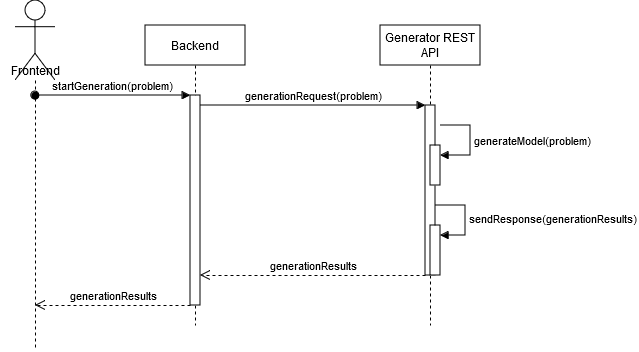
\includegraphics[scale=0.6]{include/imgs/rest_long_return.png}
				\caption{Possible long return implementation of generator REST API}
				\label{longreturnimage}
			\end{center}
		\end{figure}
		\item \textbf{Long polling:}
		Here, the REST API would respond immediately with a "Starting generator service" message, had it received the request.
		The REST API would start and perform the generation, while the backend would constantly try to fetch the results from the API.
		An example implementation can be seen in figure \ref{longpollingimage}
		\begin{figure}
			\begin{center}
				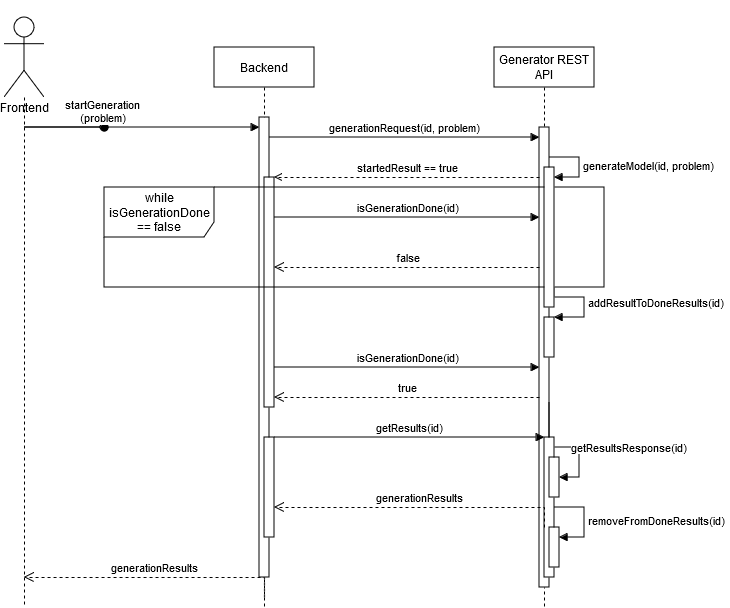
\includegraphics[scale=0.5]{include/imgs/rest_long_poll.png}
				\caption{Possible long polling implementation of generator REST API}
				\label{longpollingimage}
			\end{center}
		\end{figure}
\end{itemize}
The limitation of both implementations is the fact that the request cannot be cancelled from the client side. As that is one 
of the main requirements of the architectural restructuring (section \ref{requirements}; \ref{requirementcancel}), this 
is a fact that cannot be looked over, so I concluded that 
another architecture should be used for the implementation.


\subsection{Remote Procedure Call} \label{rpcconsiderations}
	The second architecture that came up during the designing phase was Remote Procedure Call (RPC) (section \ref{backgrpc}). 
	The generation is a procedure, so calling it remotely can free up resources from the backend server. 

	Using gRPC (section \ref{backgrgrpc}) would provide the timeout logic (section \ref{requirements}; \ref{requirementtimeout}), 
	and other clients
	could also be created in the future (section \ref{requirements}; \ref{requirementseparateclient}), 
	as the generator server would function as a gRPC server. The newly created clients would only need to
	act as a gRPC client, and send requests according to the server's specification.

	gRPC would allow us to use a one request - multiple responses implementation, for 
	representing the current state of the generation (section \ref{requirements}; \ref{requirementstate}). 

	The cancellation of the generation (section \ref{requirements}; \ref{requirementcancel}) 
	can also be done via gRPC's provided cancelation code examples. The thread running the generation of
	the model could be stopped upon receiving a cancel request.

	gRPC communicates over HTTP 2.0, so the newer HTTP protocol (section \ref{backgrhttp}) 
	would have to be used, in order to utilize the usage of the gRPC library.

\subsection{WebSocket server} \label{considerationwebsocket}
	Last but not least, comes WebSocket (section \ref{backgrwebsocket}). 
	This basically would work the same way as the REST API long polling implementation,
	however, the connection would not be closed after the initial request. This is due to the way WebSocket works.
	
	Due to the nature of WebSocket, after the model generation request is sent out by the client,
	the connection is kept alive, and the server may send back multiple responses over the same connection.
	This comes in handy for the representation of the state. (section \ref{requirements}; \ref{requirementstate})
	The server can continously send to the client,
	where the model generation is currently at. 

	The current implementation for the communication between the web client and the editor server is already using a WebSocket connection.
	As such, the same cancelation (section \ref{requirements}; \ref{requirementcancel}) and timeout logic (section \ref{requirements}; \ref{requirementtimeout})
	can be applied for the generator server, meaning that those two requirements would also be satisfied.
	After all of these considerations WebSocket seemed like the best implementation moving forward, but the way it would be implemented
	still needed to be decided:

	\begin{itemize}
			\item \textbf{Using a separate connections from the webclient side}
			This way, the webclient (or "frontend") would be the one making a connection with the generator server. This way
			there would be two connections created from the webclient: one towards the generator server, and a separate one 
			towards the editor server.

			\item \textbf{Using the same connection as the editor}
			In this implementation, the editor server (backend) would function as a "proxy" towards the generator microservice. This is made possible 
			by the fact that in the current implementation, the webclient already makes a WebSocket connection towards the editor server, and 
			the editor server is the one performing the generation.
	\end{itemize}

\subsection{Decision} \label{archdecision}
	After investigating and evaluating the possible implementations, I decided to choose the WebSocket implementaiton 
	utilizing the `backend as a proxy towards the microservice' due to the reasons below.

	The \textbf{REST API implementation} should not be used as the states where an ongoing generation stands (see section \ref{requirements} 
	requirement number \ref{requirementstate}) would be hard to represent
	without the use of a workaround. Furthermore, the cancelation of ongoing generations (see section \ref{requirements} 
	requirement number \ref{requirementcancel}) would also need some workarounds for it to be implemented.

	The \textbf{gRPC implementaiton} could satisfy all of the project requirements. The The ongoing generations could be cancelled (see section \ref{requirements} 
	requirement number \ref{requirementcancel}) and timeouts could 
	be handled too (see section \ref{requirements} 
	requirement number \ref{requirementtimeout}). 
	The gRPC implementation would introduce new dependencies for both the backend and the generator server projects.
	The final image of the backend and the generator would grow even bigger, but neither the overall user experience, performance
	or the scalability would be improved compared to the WebSocket implementation. 

	\begin{figure}[h!]
		\begin{center}
			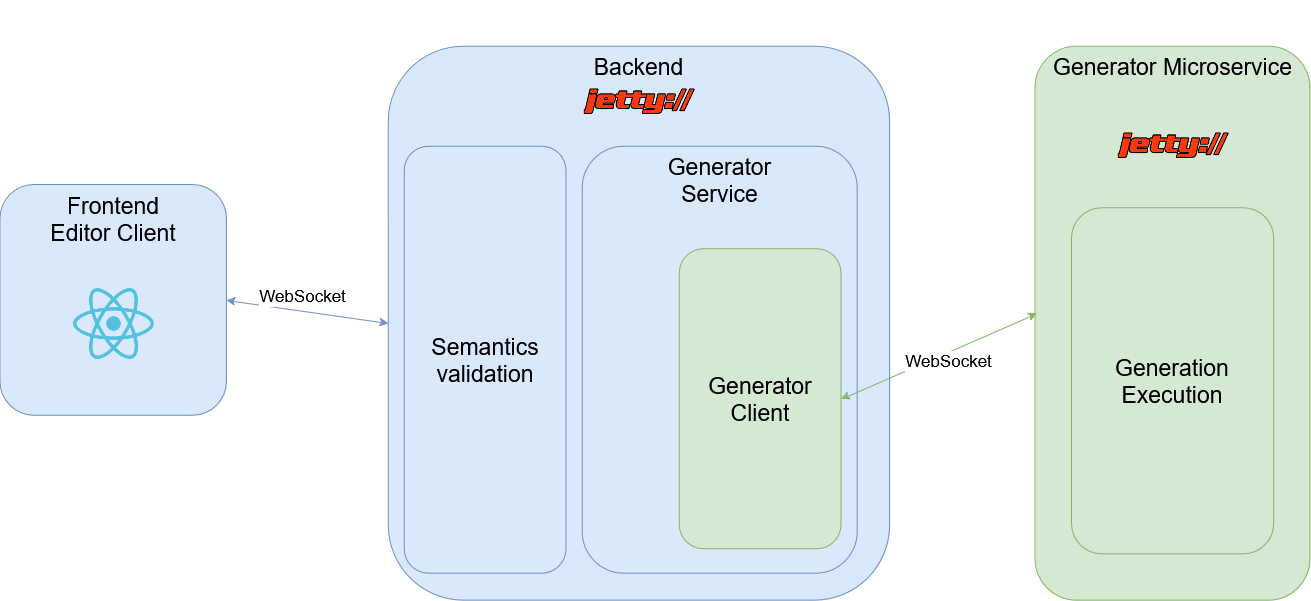
\includegraphics[scale=0.3]{include/imgs/arch_plan.png}
			\caption{Final proposed architectural changes}
			\label{archplan}
		\end{center}
	\end{figure}

	The \textbf{WebSocket implementation} proposed in figure \ref{archplan} could satisfy all of the project requirements (section \ref{requirements}). 
	Furthermore, WebSockets are already used 
	in the backend project so it should be ready to use for the microservice implementation aswell.
	This info also assures me, that there won't be any dependency issues related to this implementation. 
	Via the use of 
	WebSockets, no additional dependencies have to be added. The editor server already communicates 
	with the clients over WebSocket, through which
	the model generation requests are sent over. 
	Using WebSockets and the "backend as a proxy towards the microservice" (section \ref{considerationwebsocket}) implementation could 
	reduce the overall work needed for the refactor, 
	as the Frontend of Refinery 
	doesn't have to be touched. 
	The changes to the architecture of the application will not be noticable for the client, yet the performance may improve.

\section{Infrastructure}
	In the following sections I will describe how the modified Refinery web application could be deployed in the AWS cloud environment.

	I will utilize Amazon Web Services, as it is one of the leading industry standard cloud providers
	and the current Refinery is also deployed on AWS platforms.

	AWS currently offers many options for running our application, both server and serverless methods.
	When thinking about server methods, the ways include EC2, ECS, EKS. When talking about serverless approaches
	Fargate and Lambda are the solutions that come to mind. I'll describe how each of these
	services could be used for our infrastructure, and come to a conclusion, of how our infrastructure will be deployed.

	When deciding about the infrastructure, the key considerations are going to include the specifications for our microservice,
	how easy it is to maintain our deployed application, and last, but not least the costs affiliated with said infrastructure.


	\subsection{Elastic Compute Cloud (EC2)}
		Amazon EC2 (section \ref{backgrec2}) is the most bare-bones approach as this
		would be the same, as running a linux server on any on-prem instances. 
		By containerizing our application, no additional libraries
		would need to be installed: we just need to run our docker image, and the container would be ready to go. 
		
		Another advantage of this approach
		is the price. This is one of the cheapest services of Amazon, with instance hourly rates starting as little as \$0.0048, to going as high as 
		\$0.1728 for a single instance (key factors in pricing include CPU cores, memory and network performance).

		However, advantages of this approach stop right there. When it comes to maintaining our application, EC2 doesn't offer much.
		On the AWS dashboard, we could see, whether our instance is running, but nothing about the state of our application running in 
		the docker container. Another disadvantage, is that scaling is pretty much non-existent from the get-go. Auto Scaling Groups and Load Balancers
		can be created by using EC2 instances, but the setup of them is tedious. 

	\subsection{Serverless approaches (Fargate and Lambda)} \label{consserverless}
		Serverless options like AWS Fargate and AWS Lambda were considered for the generator application. 

		AWS Fargate offers billing based on actual usage, avoiding charges during downtimes. However, 
		its per-resource pricing (\$0.0445 per CPU core/hour and \$0.0049 per GB/hour) \cite{fargateprice} 
		can lead to higher costs compared to 
		EC2 instances, especially with increased usage.

		AWS Lambda eliminates the need for containerization and supports Java, allowing lightweight execution of code snippets. 
		Pricing is memory-based (e.g., \$0.0000000083 per ms for 512MB in Europe) \cite{lambdaprice}, which seems cost-effective. 
		However, Lambda is better suited for lightweight tasks, and its performance may degrade under heavier workloads. 
		Moreover, its stateless nature complicates tracking generation states, user-requested cancellations, and 
		integration with the backend and frontend.

		Both Fargate and Lambda scale well, but serverless solutions do not align with key application requirements
		(e.g.: section \ref{requirements}; \ref{requirementstate}, \ref{requirementcancel}, \ref{requirementtimeout}).
		The ease of migration to other cloud providers or local deployments would also be lost. 
		These limitations outweigh potential cost savings for low usage, leading to the decision to forgo a serverless approach.
		

	\subsection{Elastic Container Services (ECS)}
		With Amazon ECS (section \ref{backgecs}) tasks can be run using EC2 (section \ref{backgrec2}) or AWS Fargate instances.
		The amount of vCPUs and memory allocated for each container can also be configured.
		Setting up an ECS cluster has no additional costs affiliated with it, other than the cost of the running EC2 or Fargate instances.

		Scaling can be made possible via the usage of auto scaling groups (section \ref{backgautoscaling}) and load balancers 
		(section \ref{awslb}). Within auto scaling groups, we can define how many
		running instances we want to allow our services to scale up to. The triggering effects can also be set, such as average CPU utilization and 
		average memory usage. If our task reaches that treshhold, a new instance of the task is launched.  
		The load balancers immediately register the running instances within the auto
		scaling group, so that would also make the implementation pretty straightforward. The load balancer can forward traffic to generator 
		microservice instances based on their routing algorithm, which can either be set as a round-robin or least connections.

		ECS also helps the maintanence of the infrastructure. AWS can collect many logs associated with 
		the container tasks. Monitoring of the resource usages can also be done via AWS management console dashboards.

		Due to the drawbacks of a serverless implementation listed in section \ref{consserverless}, it would be beneficial to use EC2 instances
		for the running of our containers. That implicates that the implementation has to be done in a way, where our generator
		microservice docker container (section \ref{Docker images}) acts as a server.

	\subsection{Kubernetes}
		Kubernetes could be used as a tool for container orchestration, without the need of any provisioning tools. 
		However, the project is mainly related to the creation of a generator
		microservice and removing the generation from the main backend. As a result, using 
		Kubernetes or Elastic Kubernetes Service (EKS) for this task
		would be way too overkill, as only two containers would be running at the same time. 
		For a task of this size, the YAGNI principle (= `You are not gonna need it') should be applied.
		
		EKS wouldn't even allow us to become more independent
		from the AWS infrastructure. However, if using another 
		public cloud provider was an aspect that we would need to consider, this would be a viable option. Kubernetes also allows for 
		greater customizability of auto scaling properties.

	\subsection{Decision} \label{awsdecision}
		The final deployment of our infrastructure will be done via the use of ECS and EC2 instances running the defined container tasks.
		The tasks should be running on the same auto scaling group of EC2 instances. 
		
		A load balancer will be added, so that the 
		network traffic can be forwarded to the tasks running our docker containers. The cost of an application load balancer is \$0.02394 per Application 
		Load Balancer-hour in the Stockholm region, where I am planning to deploy the application in the future. This application load balancer
		will balance the traffic towards basic backend target groups, and also towards generator server instances.

		Another key factor, is that Amazon has cheaper prices for EC2 instances with arm cpu architecture. It would be beneficial
		to create a multi-architectural docker images, so that when we deploy our application, cheaper running costs can be 
		achieved.

		With this plan, using t3a.micro arm EC2 instances, the costs associated with the deployment should be as follows:
		
		\begin{center}
			Minimum cost per hour = $2 \times \$0.0108$ + \$0.02394 = \$0.04554
		\end{center}

		So approximately 4.6 cents per hour. This includes the usage of two EC2 instances and an Application Load Balancer.

		\begin{figure}[h!]
			\begin{center}
				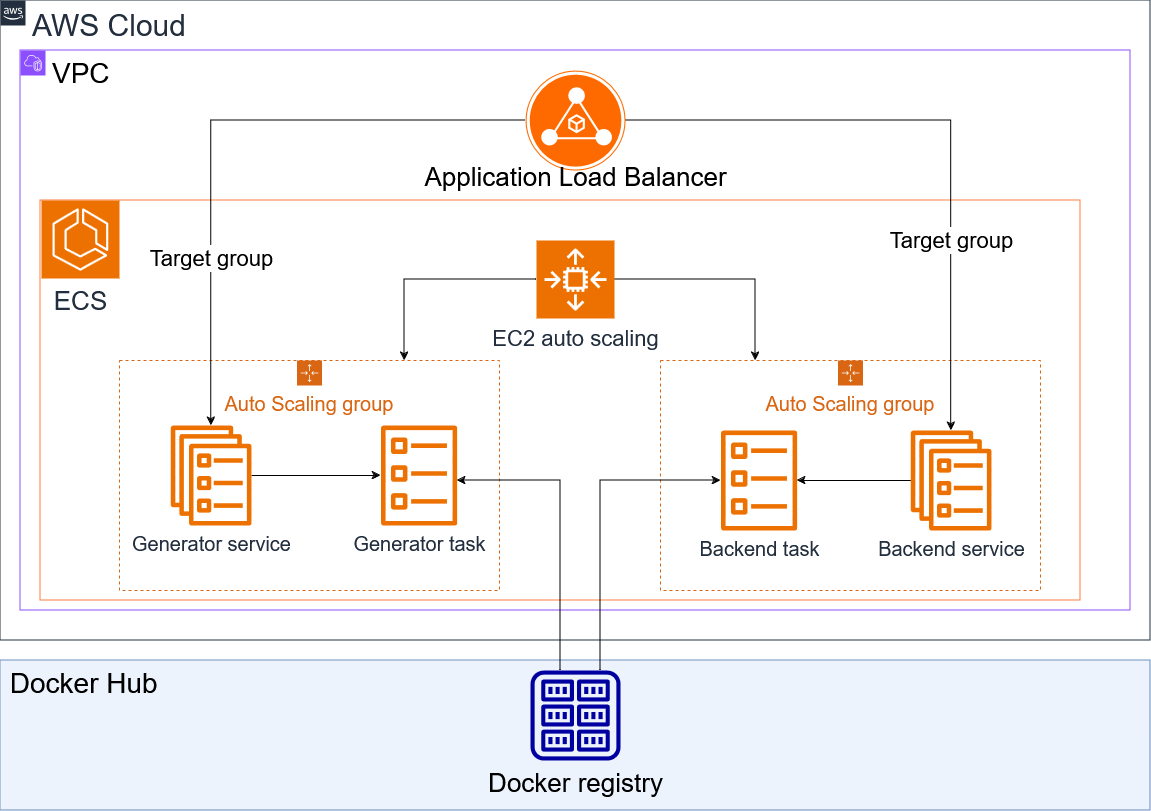
\includegraphics[scale=0.35]{include/imgs/aws_infra_plan.png}
				\caption{Final proposed infrastructure for deployment}
				\label{infraplan}
			\end{center}
		\end{figure}
\chapter{Implementation} \label{Implementation}

	This chapter delves into the implementation of the planned architecture defined in section \ref{archdecision}.
	First I will introduce the starting point of the project.
	Then I will go into detail about the implementation of a client within the backend, which communicates with 
	the generator microservice. Finally I will go into detail
	regarding the inner workings of the generator server.

	The starting backend's class diagram can be found in the appendix at \ref{startingbackenduml}.
	The implemented generator client can be seen at \ref{backendclientuml}.
	The implemented generator microservice can be seen at \ref{generatorserveruml}.

	\section{Starting point} \label{Starting point}
		First, I will introduce the starting point of the project, so we get an overview, of how the backend initially worked regarding the model
		generations.

		The PushServiceDispatcher is the class responsible for calling the functions of the ModelGenerationService instance, and thus initiating
		the generation related methods.

		\subsection{ModelGenerationService} \label{ModelGenerationService}
			The \textit{ModelGenerationService} is a core component of the application, designed to handle the starting and management of
			model generation workers (section \ref{ModelGenerationWorker}) on the backend server. 
			It is a singleton class, so from a generator point of view, we might consider this class to be the real dispatcher.

			The key features and responsibilities of the class include:
			\begin{itemize}
				\item{\textbf{Service Initialization:}} The \textit{ModelGenerationService} is a singleton, 
				ensuring a single, consistent instance throughout the application's lifecycle.
				It retrieves configuration parameters such as the model generation timeout 
				from the environment, defaulting to 600 seconds if not explicitly set.
				\item{\textbf{Model Generation Workflow:}} The main responsibility of the service is to execute model generation requests 
				by instantiating workers (\textit{ModelGenerationWorker}), using multithreading. The amount of threads 
				where the workers can be run is set via an environment variable (REFINERY\_MODEL\_GENERATION\_THREAD\_COUNT 
				\cite{generationthread}).

				The service interacts with the document’s \textit{ModelGenerationManager} to monitor the workers.
				The timeout and cancellation is handled via the use of cancelation tokens.
			\end{itemize}
			The use of dependency injection for worker provisioning ensures that the service is decoupled from the specific implementation details
			of task execution, making it easier to extend or modify in the future.

		\subsection{ModelGenerationWorker} \label{ModelGenerationWorker}
			The \textit{ModelGenerationWorker} class is where the actual model generations happen. 
			It operates as an independent thread, processing generation requests in a thread-safe and scalable manner. 
			Its multithreaded design uses Java's ExecutorService to manage task execution efficiently within a threadpool.

			Each worker instance is uniquely identified by their UUID. Before execution, the worker’s state is configured 
			with essential inputs, such as the document containing the generation request, a random seed, and a timeout value. 
			This sets up the generation and prepares the worker for execution.

			The worker’s primary responsibility is to handle the computational workflow, 
			which includes parsing the input into a formal problem, generating a solution, extracting metadata, 
			and converting results into a JSON (section \ref{backgrjson}) format. 
			Throughout this process, the worker monitors for cancellation requests and timeout. 

			Once a task is completed, the worker notifies the service whether the generation was successful or ran into an error. 

	\section{Generator Client} \label{Generator Client}
			Now that the deployed implementation has been been described, we can restructure our application, so that the 
			model generation is done via the generation microservice.

			The design of the \textit{ModelGenerationService} (section \ref{ModelGenerationService}) is scalable and modular:
			By delegating the actual computation to workers (ModelGenerationWorker, section \ref{ModelGenerationWorker}), 
			the service separates dispatching and execution. 
			
			This comes in handy, when implementing our client for communication with
			the generator server. We have to implement a client, which communicates generation requests towards the generator server,
			and upon completion, receives such generation results.

			The implemented client's UML class diagram, alongside the modifications to the backend can be seen in appendix \ref{backendclientuml}.

			\subsection{GeneratorWebSocketEndpoint} \label{GeneratorWebSocketEndpoint}
				This class is responsible for sending generation requests and handling responses is implemented as the 
				GeneratorWebSocketEndpoint class,
				using Jetty's WebSocket API (section \ref{backgrjetty}). 
				This endpoint facilitates asynchronous communication with the generator microservice, 
				ensuring efficient request management over WebSocket connections. 

			In the following sections, I will describe the key responsibilities and functionalities of the GeneratorWebSocketEndpoint class.
			\subsubsection{WebSocket Configuration} 
				The server, which the client is communicating with, can be configured.
				\begin{itemize}
					\item The WebSocket URI is dynamically determined based on environment variables (\textit{REFINERY\_GENERATOR\_WS\_HOST} 
					and \textit{REFINERY\_GENERATOR\_WS\_PORT}). If these are unset, default values (localhost and 1314) are used to ensure flexibility during deployment.
					\item The constructor initializes a WebSocketClient instance and sets default values, such as the worker's UUID and timeout duration.
				\end{itemize} 
			\subsubsection{Communication towards the server} 
				\begin{itemize}
					\item The client connects to the server via a ClientUpgradeRequest. The connection includes a custom header for the UUID of the worker.
					\item Sending the generation requests via sendGenerationRequest method. The method sends a structured JSON payload containing the request type,
					the UUID, the problem description, and a random seed. This start the model generation process on the server
					\item \label{clientcancel}Sending generation cancel requests via the sendCancelRequest method. This client sends a JSON, with the UUID of the generation to be 
					executed. Each generation opens a new session, with a new UUID for the server, so they can be uniquely idenfitied.
				\end{itemize} 
			\subsubsection{Receiving from the server} 
				Responses from the server are handled by the onText method, which processes various types of messages 
				(result, error, nodesMetadata, relationsMetadata, partialInterpretation), parsing them into appropriate data 
				structures and queuing them for consumption in their appropiate result queues (section \ref{resultqueues}).

			\subsubsection{Parsing responses from the queue} \label{resultqueues}
				The client maintains several LinkedBlockingQueue instances to manage received data:
				\begin{itemize}
					\item responseQueue: Stores results or errors associated with the generation process.
					\item nodesMetaDataQueue: Holds metadata about nodes in the generated model.
					\item relationsMetadataQueue: Queues relation metadata details.
					\item partialInterpretationQueue: Handles intermediate model interpretation data.
				\end{itemize} 
				The queues are accessed with timeout constraints to prevent indefinite blocking during retrieval. The timeout is set up by the class's
				timeout variable. 
				
				The LinkedBlockingQueue allowed the onText method, to put the received generation
				results into the queue, while the client is waiting for the results to arrive from the server. As soon as an element is put into the queue
				it can be popped from it. This way our code is safely waiting for the results
				to arrive from the server and no concurrency issues can arise. As I have already mentioned, each generation request instantiates a new
				client, so the size of these queues can only be between 0 and 1. No other generation client is accessing these queues of the instances.


		\subsection{ModelRemoteGenerationWorker} \label{ModelRemoteGenerationWorker}
			\subsubsection{Core functionality}
				The ModelRemoteGenerationWorker manages the WebSocket client (section \ref{GeneratorWebSocketEndpoint}) in a multithreaded
				fashion. The class operates with the same threadpool introduced in section \ref{ModelGenerationWorker}. This way, the old 
				local generation (section \ref{ModelGenerationWorker}) could be replaced with this remote client, 
				with no other major changes done to the codebase.

			\subsubsection{IGenerationWorker}
				For implementation, the IGenerationWorker interface was created, which defines a unified API for all generation workers. 
				This interface standardizes the core operations, including task initialization, execution, timeout management, and cancellation.
				This abstraction ensures that the backend can switch between local and remote workers. The switch can be toggled via
				an environment variable. The old ModelGenerationWorker and the ModelRemoteGenerationWorker both implement this interface.

				The key methods from the interface include:
				\begin{itemize}
					\item setState: Configures the worker with the input document, random seed, and timeout settings.
					\item start and startTimeout: Enqueues the worker for execution and schedules a timeout to enforce task completion within a defined duration.
					\item doRun: Executes the remote model generation logic by communicating with the external service.
					\item \label{workercancel}cancel: Cancels the task, ensuring both local and remote operations are halted gracefully.
				\end{itemize}

			\subsubsection{Workflow}
				The execution process of ModelRemoteGenerationWorker begins with setup and state configuration. 

				During task execution, the worker sends a generation request to the remote service by using a WebSocket client instance (GeneratorWebSocketEndpoint). 
				The server's responses are processed incrementally.

				The task completes successfully upon retrieving all necessary results, or it is terminated on errors, cancellation, or timeout.

				Timeouts and cancellations are managed via a ScheduledExecutorService, ensuring that the system remains responsive and resources are freed promptly. In case of errors, the worker captures exceptions, logs the issues, and notifies the backend with appropriate error results.

				The interaction between the GeneratorWebSocketEndpoint and the ModelRemoteGenerationWorker 
				showcases how client-side operations are integrated into the existing codebase.

	\section{Generator Server} \label{Generator Server}
		Now that the client side of the generation process has been introduced, the server side implementation is what should be described next.
		The main idea behind this implementation, was to take the experiences of the local model generation worker, and basically implement everything that 
		is necessary for a generation to happen, in a multithreaded way, on our microservice. It is basically the implementation of 
		the ModelGenerationWorker (section \ref{ModelGenerationWorker}) on a separate server.

		The UML class diagram of the Generator Server can be found in the Appendix at \ref{generatorserveruml}.

		\subsection{GeneratorServerEndpoint} \label{GeneratorServerEndpoint}
			The GeneratorServerEndpoint is a WebSocket server endpoint utilizing Jetty's WebSocket server API \ref{backgrjetty}. 
			The server actively listens
			to generation requests and upon receiving submits the requests to the ModelGeneratorDispatcher 
			(section \ref{ModelGeneratorDispatcher}).

			\subsubsection{Core Functionality} \label{Core Functionality}
				The two most important functionalities of the class are the handling of the generation requests and cancelation requests, which are
				 received over the 
				WebSocket sessions. 
				
				When a message of type `generationRequest' is received, the endpoint extracts generation details 
				such as the unique identifier (UUID), random seed, and problem description. The data is sent by the client (section \ref{GeneratorWebSocketEndpoint} 
				and section \ref{ModelRemoteGenerationWorker}) via JSON, so extracting the
				needed key-value pairs is straighforward. These are then forwarded to the ModelGeneratorDispatcher, 
				which manages the actual model generation task.

				\label{serverendpointcancel}For `cancel' messages, the endpoint instructs the ModelGeneratorDispatcher to cancel an ongoing generation task associated with the provided uuid.

				Any errors during the WebSocket communication are captured, logged.

				When a WebSocket session is closed, the endpoint notifies the ModelGeneratorDispatcher to clean up resources associated with the disconnected client.

			\subsubsection{Integration into the workflow} \label{Integration into the workflow}
				The GeneratorServerEndpoint serves as the entry point for remote clients into the generator microservice. 
				It relies on the ModelGeneratorDispatcher to manage generation and cancellation tasks. This provides a clean separation of concerns. 
				The design ensures that the endpoint focuses solely on communication, while the dispatcher handles the generation tasks.

			\subsubsection{Scalability and Extensibility} \label{Scalability and Extensibility}
				This WebSocket-based implementation allows the backend to support multiple concurrent client connections efficiently. 
				By using asynchronous communication, it ensures that tasks are queued and processed without blocking the ongoing generations. 
				The modular design makes it easy to extend functionality, such as adding new message types or enhancing error handling mechanisms.


		\subsection{ModelGeneratorDispatcher} \label{ModelGeneratorDispatcher}
			The ModelGeneratorDispatcher is a singleton class designed to manage and execute model generation requests on separate threads. 
			Its primary role is to coordinate the model generation tasks, making sure that they run concurrently. 
			This dispatcher simplifies the handling of multiple requests 
			and helps with maintaining system consistency.

			\subsubsection{Key features} \label{Key features}
			The class implements the singleton design pattern to guarantee that only one instance of ModelGeneratorDispatcher exists throughout the application. 
			This is achieved via the use of a private constructor which prevents instantiation of the class from the outside, ensuring 
			that all interactions go through the singleton instance.
			This provides centralized control and avoids conflicting task management.

			The GeneratorServerEndpoint submits the received generation requests for this class. 
			Each model generation request is executed in a separate thread. 
			This is achieved through the ModelGeneratorExecutor (section \ref{ModelGenerationExecutor}) class, which handles the task logic.
			The running model generations (ModelGenerationExecutor) are stored in a hashmap. The processing threads are identified by 
			the UUID of the generation in the hashmap.

			\label{servercanceldispatcher}Ongoing tasks can be cancelled via the UUID of the generation. As the hashmap stores these generation tasks identified by their UUID, it is fairly easy to do so.

			Once a client has disconnected, the belonging task is cancelled, if not finished yet. The said task is removed from the hashmap. The UUID identification is 
			useful here aswell.

		\subsection{ModelGeneratorExecutor}\label{ModelGenerationExecutor}
		The ModelGeneratorExecutor is a class responsible for performing the actual model generation tasks. It runs on a separate thread, 
		making it suitable for concurrent processing. This class does what the original ModelGenerationWorker 
		(section \ref{ModelGenerationWorker}) did in the original implementation. 
		It even operates as part of a dispatcher system. The running of these executor threads is started by the ModelGeneratorDispatcher 
		(section \ref{ModelGeneratorDispatcher}).

		\subsubsection{Key features and responsibilities}\label{Key features and responsibilites}
			The main responsibilites of the class are the following:
			\begin{itemize}
				\item \textbf{Initialization:} Before starting, it initializes the problem by loading the problem description, random seed, and WebSocket session details. These were
				received by the GeneratorServerEndpoint over WebSocket, and are given to an executor object by the ModelGeneratorDispatcher.
				\item \textbf{Task Execution:} The class handles the execution of the model generation. This is done in the exact same way, as it was done previously at the local ModelGenerationWorker.
				\item \textbf{Client communication:} By receiving an open WebSocket session in the constructor, the class instance can send generation 
				state results, metadata and errors to the clients.
				\item \label{serverexecutorcancel}\textbf{Cancellation support:}The task can be interrupted or canceled at any point, 
				making sure that unnecessary processing is avoided. This is especially useful for timeout scenarios or user-initiated cancellations.
			\end{itemize}

		\subsection{ServerLauncher}\label{Serverlauncher}
		The ServerLauncher class serves as the entry point for starting a WebSocket server that 
		processes model generation requests (section \ref{GeneratorServerEndpoint}). It listens on a configurable port, defaulting to 1314 
		unless overridden by the \textit{REFINERY\_GENERATOR\_WS\_PORT} environment variable. 
		
		The class sets up a Jetty server, running the implemented GeneratorServerEndpoint.
		Once everything is configured, the server is started to handle incoming requests. 
		This class essentially establishes the server infrastructure for the application.

	\section{Containerization}\label{Containerization}
		The new generator microservice was added 
		to the `run' task of the backend Gradle project, and as such, the workings of the application could be tested locally in a manual fashion. 
		
		Containerization (\ref{backgcontainer}) was the next step in 
		updating our application. 

		Even before the restructuring, the build pipeline already existed. My main task was integrating the generator server docker image creation
		into these available scripts of the pipeline. 

		\subsection{Preparation scripts}\label{Preparation scripts}
			The process begins with a build script that compiles the project's distributed components, such as the backend and generator microservices, into portable archives. 
			This is done via the use of Gradle (\ref{backgrgradle}).

			One script organizes and optimizes the build outputs, ensuring shared dependencies are deduplicated and arranged for efficient reuse. 
			It also prepares architecture-specific resources to support multi-architecture Docker builds, arranging all necessary files into a structured context for image creation.
			I had to modify this script, so that it also handles the same process for the newly created generator server's (\ref{Generator Server}) archives.

			Finally, a dedicated script builds and optionally pushes Docker images using a multi-stage build configuration. 
			This configuration leverages tools like Docker Buildx and supports deployment across different architectures, ensuring compatibility. 

		\subsection{Docker images}\label{Docker images}
			The project utilizes a structured and reusable approach to Docker (\ref{backgdocker}) image creation, leveraging a common base image and architecture-specific 
			optimizations to support multi-architecture compatibility.

			A configuration file specifies the group of targets (like the base, backend and generator) and individual build configurations for each target. 
			These targets are the created docker images.

			These targets share a lightweight base image that includes essential runtime dependencies. 
			Each target builds on this foundation, adding service-specific layers such as dependencies, binaries, and configuration files.

			I implemented the Dockerfile.generator to containerize the generator service efficiently. It builds the service using a multi-stage process, 
			layering runtime dependencies, application files, and configuration (like environment variables and exposed ports). 
			It uses the base image as its starting point.

			I also created a Docker Compose (\ref{backgdockercompose}) file for the local deployment of the application. Via this, the manual testing of the 
			created application docker images can be done. Before deploying to the production infrastructure, this can add an extra layer of ensuring proper workings.

			The finished images were pushed to the Docker Hub registry. The public repository containing the images (backend,
			generator) can be accessible by anyone, and are needed for the AWS deployment.


	\section{Deploying on AWS} \label{awsdeploy}
		In this section I will describe the deployment of the modified Refinery backend and the Generator microservice. The deployment will be 
		done according to the plan setup in \ref{awsdecision}.

		I registered a new AWS account with my own private email address.
		For the creation of the infrastructure I used the AWS Management Console, which is the web GUI for 
		managing our AWS infrastructure.

		\subsection{Task definitions} \label{awstasks}
			First I set my tasks up. The tasks are basically the container instances of an application within the AWS ECS environment. 
			I created a task
			for the generator microservice called refinery-generator and the backend server called refinery-language-web.
			In the task configuration, I set the tasks to run on EC2 instances, provided the belonging docker registry link for the service,
			assigned the port mappings for the appropiate listening ports, and set the environment variables, 
			such as the generation host and port. The refinery-language-web task definition needed the `REFINERY\_GENERATOR\_WS\_HOST' to 
			be equal to the load balancer of the generator microservice's load balancer (this had several issues as explained 
			in section \ref{ALB NAT}).
			I set the networking mode for both tasks to be awsvpc, as they would be deployed on the same Virtual Private Cloud.
			Health checks also had to be implemented, so that our service knows, that the application is running and is in a stable state.
			For health checks, I used basic curl requests to the host and ports of the services. This needed modification for 
			the generator server codebase (section \ref{healthcheck}).

		\subsection{Service definitions} \label{awsservices}
			I created a refinery cluster, with services running the defined tasks in \ref{awstasks}. The services are within an 
			EC2 auto scaling group. 
			This allows us to scale our container instances, if they are heavily used and the resource usage is over a threshold.
			For this I set up two treshholds:
			\begin{itemize}
				\item CPU usage: If the average CPU usage is over 70\% for more than 300 seconds, a new instance is deployed.
				\item Memory usage: If the average RAM usage is over 70\% for more than 300 seconds, a new instance is deployed.
			\end{itemize}
			I used Amazon's t3.micro EC2 instances for the auto scaling group, which are eligible for the free tier accounts. 
			They each have 2 vCPUs with 4 threads and 1GB of RAM.
		
		\subsection{Load Balancer definition} \label{awslb}
			An application load balancer (ALB) was created for the 
			backend and the generator server. The ALB would forward traffic to the running container instances within a target group, as longs as their
			health checks pass. 
			The ALB would be reachable for anyone on the internet on port 80. This port forwards traffic to the target group of the backend of the application.
			On port 81, the forwarding of the generator microservice requests is done towards the generator target group. However, this port is configured
			to accept requests only within the security group of the application. As such, only the backend can send requests to the microservice, hiding it 
			away from the public internet.
			I set the load balancing algorithm to the default round-robin, but least-used can also be a viable option.

	\section{Challenges during the implementation} \label{challenges}
	\subsection{Resource usage of development}
		I wanted to develop on the Linux operating system, via the use of Windows Subsystem for Linux (WSL). WSL was needed because 
		of the build scripts, which were implemented for UNIX shells.

		When I initially opened the Refinery gradle project via a remote connection to my WSL the resource usage 
		for the gradle project indexing was huge. The 8-core Ryzen 7 CPU was sitting at around 70\%  usage, alongside 
		16 gigabytes of my system memory being 92-99\% occupied. 
		
		The initial indexing of the Gradle project took around 45-60 minutes. Even upon completion the resource usages did not improve. 
		The same amount of RAM
		was used by the WSL and it would not become lower. 

		\begin{figure}[h!]
			\begin{center}
				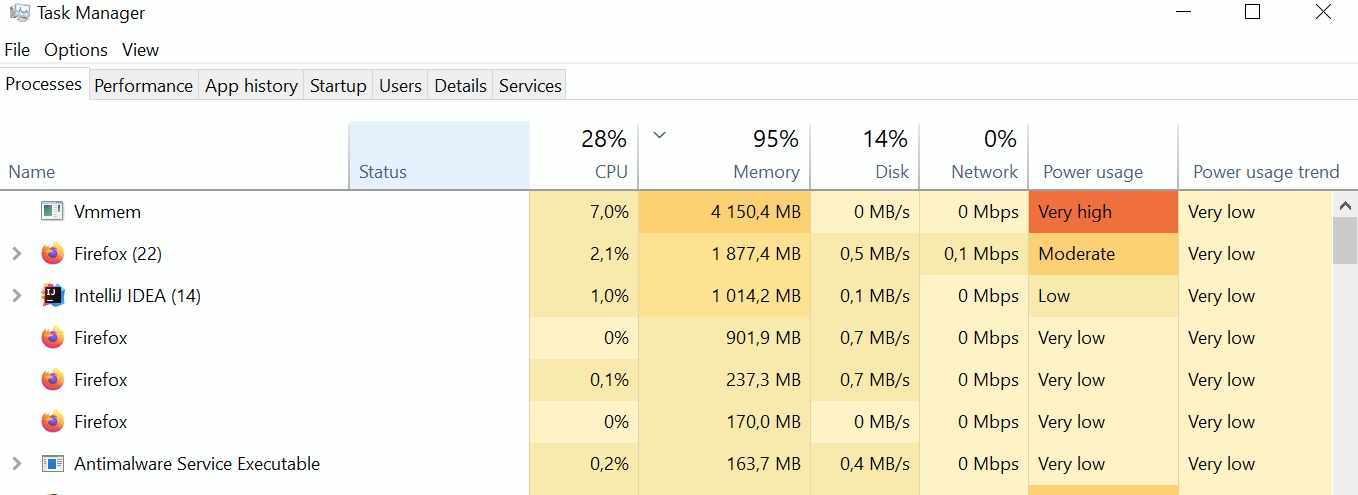
\includegraphics[scale=0.35]{include/imgs/res_usage.jpg}
				\caption{Resource usage during developing on WSL}
				\label{resourceusagewsl}
			\end{center}
		\end{figure}

		As a result of this, I have given up on the development using WSL. I developed the application on Windows, while using WSL only for the
		dockerization (\ref{Containerization}) of the finished applications.

	\subsection{Deduplication for docker images}
		The initial context preparation in section \ref{Preparation scripts} was implemented for two different distributions (the basic backend 
		named web, and a generator cli called cli). The common\_libs creation for both of these distributed images was straightforward
		as the two distributions only had limited amount of JARs that they both used.

		With my project, a new distribution for the generator server was created. Originally I wanted to implement the deduplication in a way,
		where if two of the three distributions contained a JAR, the JAR would be put in the common\_libs folder.
		However, this implementation did not seem useful. In this case all of the resources needed for the web distribution were added to the common folder.
		As such, the shell script would have needed to be modified aswell, so that it could handle empty dist folders during the pipeline. 
		On the other hand
		all of the files from the common library would be put in the base docker image, even tho it might not be needed for the 
		running of our application. This would risk the bloating of the base image.

		I decided to add only those resources to the common library, which are used in all of the created docker images. 
		As a result, the base image is not bloated and the shell script did not need many modifications.

	\subsection{Health check for the generator server} \label{healthcheck}
		When deploying an application with the use of an Application Load Balancer, a target group of the tasks has to be specified.
		The load balancer needs to keep track of the running task docker container instances, so that it can decide, whether requests can be 
		forwarded to the running microservice. A health check has to be put in use, so that the load balancer can register the running instances.

		In my implementation of the generator server at section \ref{GeneratorServerEndpoint}, I only created a WebSocket server. However, Jetty 
		WebSocket servers would not respond to regular HTTP requests. With this original implementation, the health check for the load balancer would
		not work: it always signaled that the task was not running, as it would not respond to the curl http requests towards the default path (/).

		As a workaround, I created a servlet called HealthCheckServlet, which responds to HTTP get requests (section \ref{backgrhttp}) at the path `/healthcheck',
		by returning a `Server works!' plain text.

		I added the servlet to the ServerLauncher of the generator microservice. By this, the load balancer can ensure the healthy state of the 
		the server instances, by sending a curl request to the `/healthcheck' path of the generator server.

	\subsection{Application Load Balancer and NAT} \label{ALB NAT}
		During the deployment process, I faced persistent issues with the backend failing to connect to the generator microservice 
		through the Application Load Balancer (ALB), resulting in request timeouts. Initially, I suspected an Access Control List (ACL) 
		issue within the VPC hosting the infrastructure. To rule this out, I configured the ACL to allow all inbound and outbound traffic 
		and ensured Security Group policies were set to restrict access to the generator microservice only from the backend server. 
		Despite these changes, the issue persisted, with the backend unable to connect to the ALB's DNS.

		To further investigate, I accessed the EC2 instances running the ECS tasks by configuring an SSH key pair. 
		Using tools like curl and ping, I confirmed the EC2 instance could communicate with the ALB, including receiving expected responses 
		from the generator microservice's health check endpoint (\ref{healthcheck}). However, when testing connectivity from within the container 
		using a statically compiled curl binary, no response was received from the ALB.

		Through further research, I identified the root cause: ECS tasks using the awsvpc network mode are assigned private IP addresses, 
		while the ALB has only a public IP address. Since AWS does not perform Network Address Translation (NAT) within the VPC, 
		the ECS tasks could not directly reach the public ALB. This required implementing a solution to perform the necessary address translation, 
		ensuring proper communication between the backend and the generator microservice.

		\begin{figure}[h!]
			\begin{center}
				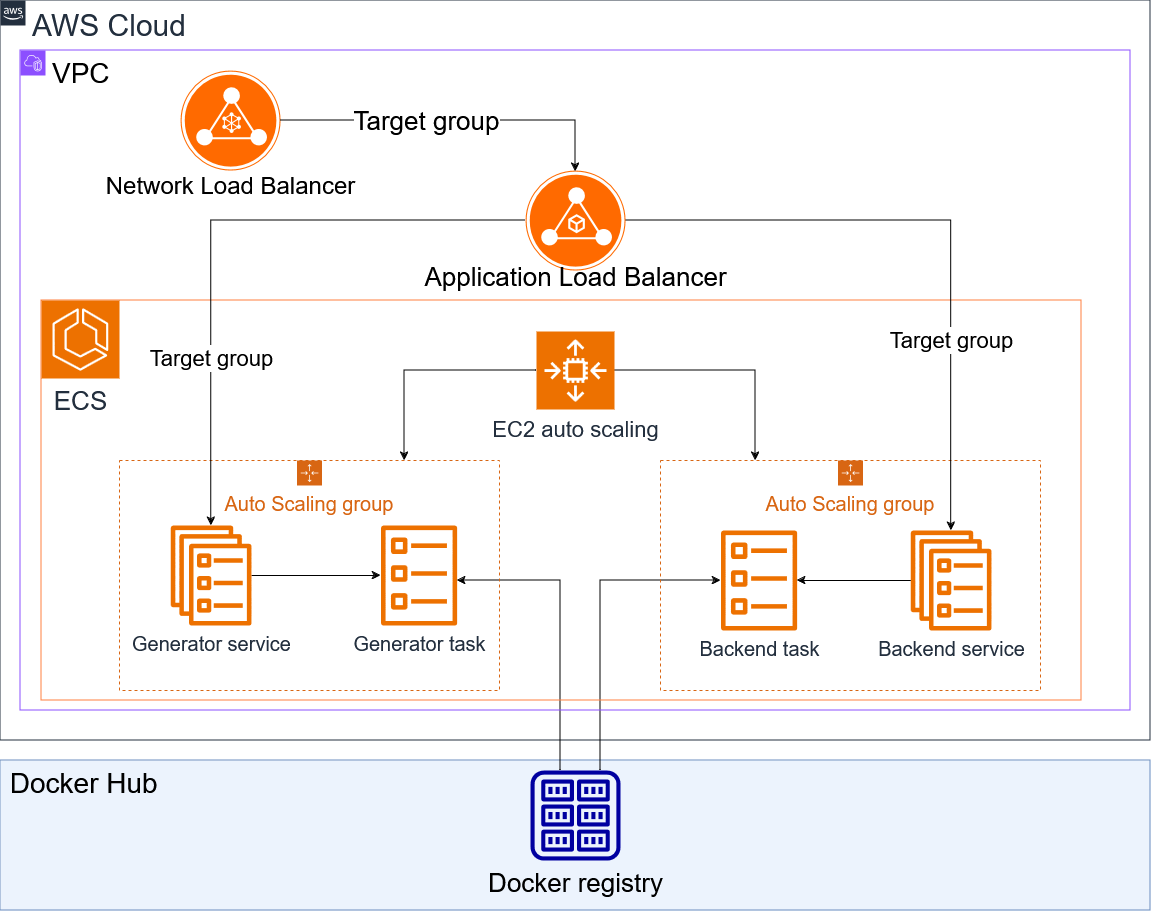
\includegraphics[scale=0.35]{include/imgs/final_aws_infra.png}
				\caption{Final deployed infrastructure}
				\label{infrafinal}
			\end{center}
		\end{figure}

		I faced two options to address the public-private IP connectivity issue: setting up a Network Load Balancer (NLB) or a Network Address Translation (NAT) gateway.

		The NLB, like the ALB, operates using target groups but supports private IPv4 addresses. 
		By configuring the NLB to use the ALB’s public IP as a target, the NLB effectively serves as a NAT solution, enabling private ECS tasks to communicate with the ALB. 
		Alternatively, the NAT gateway would facilitate communication between services across public and private subnets and provide greater flexibility 
		for future infrastructure expansions, even outside AWS.

		I chose the NLB due to its lower cost. The NAT gateway has a fixed hourly rate of \$0.046 (\cite{natprice}), whereas the NLB’s cost is traffic-dependent (\cite{nlbprice}). 
		Based on AWS’s pricing examples, the NLB was projected to cost nearly half as much under lower traffic conditions. 
		To finalize the setup, I updated the backend task configuration to point the REFINERY\_GENERATOR\_WS\_HOST environment variable to the NLB's DNS. 
		The completed infrastructure setup is illustrated in Figure \ref{infrafinal}.
\chapter{Evaluation}

	\section{Requirement analysis}
	In this section I'll go over the requirements that were made before the beginning of the project (\ref{requirements}) 
	and showcase how each of them are satisfied.

	The backend of the application is scalable in several ways. The most obvious one, is how the application is deployed on AWS. 
	If the resource usages hit a certain treshold, a new task is deployed. If the task cannot fit on an already running EC2 instance,
	the running EC2 instances scale up. This was desribed in section \ref{awsdeploy}. The other way the application supports 
	scalability is the way it handles multiple generation requests. Both the server (\ref{Generator Server}) and the client
	(\ref{Generator Client}) for the generator 
	functionality support multithreaded operation. As a result, generation requests can run in parallel, and the resource utilization
	is improved.

	The generation can be cancelled. The backend sends cancellation requests to the generator server (\ref{clientcancel}).
	When the generator server receives a cancel request (\ref{serverendpointcancel}), it instructs the dispatcher 
	(\ref{servercanceldispatcher}) to cancel the generation on the executor (\ref{serverexecutorcancel}).

	The frontend is able to show the state of the model generation. The states are sent by the generator server's executor via
	the open session to the clients.

	There is a timeout set for both the backend generator client and the generator server. This insures that even is some kind of 
	unexpected operation happens, the generation won't be stalled and use resources in a locked state.

	The editor and the generator can be deployed together. During development phase, the backend and the generator server can be 
	deployed together, via the gradle "run" task. This starts running both the generator microservice and the backend locally.
	Other than that a docker compose file was written, so that the containerized applications can be run locally.

	One optional requirement wasn't satisfied by this implementation. The creation of other type of clients other than the browser
	based one is possible, but tedious. My testing python script basically acts as a different client, but it replicates the WebSocket
	messages of the frontend client, in order to create an editing session and send generation requests.

	The price of the hosting has changed due to the issues described in \ref{ALB NAT}. The price of the deployment for an hourly rate 
	is expected to be:

	TODO WRITE THE FREAKING PRICE!!!

	\section{Benchmarks}
		\subsection{Test setup}
		I wanted to test, whether the response times of the deployed application really improved with the modifications.

		I wrote a Python script replicating the WebSocket messages of the Refinery frontend. First it creates the connection
		towards the server. Then sends the initial update
		of the example text, that can be seen in the editor at start. Then a generation request is sent to the backend and the start time of the generation
		is logged. When all of the generation results have arrived and none of them is an error, the end time of the generation is logged. 
		The script is implemented in a way, where it can run in a multithreaded way. I can send out as many simultaneous generation requests 
		from as many python clients as I'd want to. In this test, I'll send out 1, 25, 50, 75, 100, 125, 150, 175, 200, 225 generation requests
		at the exact same time, and see how the response times improve.

		The running of the python test client could be done on an Amazon EC2 instance or on a personal computer. I have decided to run the test 
		from my own personal computer, as this provides a more accurate representation of the real usage of the application.

		The tests were performed with two t3.micro EC2 instances running at the start. These VMs have 2vCPUs and 1GB of memory. I allocated
		2vCPUs and 0.9GBs of memory for each task. Since I was running two services, with the forementioned task configurations, 
		those wouldn't be able to fit on a single EC2 instance. The auto scaling acted accordingly, and deployed the services on two 
		separate EC2 instance. 

			\subsubsection{External threats to validity}
			Since the infrastructure is deployed on Amazon's infrastructure, the availability of the service and the communication speeds between the two services 
			depend on Amazon's network. As the results cannot be 100\% accurate, repeated testing should be
			performed.

			The network speeds are not constant and can be very volatile during the period of the test. The upload and download speeds of my computer, running the 
			python test client can also make some test data dirty / invalid.  Repeated testing should also solve this threat.

			The load balancer for the backend allows accepts traffic from anything on the public internet. Although the chance of it is really low
			but denial of service attacks migth invalidate the results of the test. I tried to lower the chance of this happening, by applying a security group
			to the load balancer for the duration of the test. With this, the load balancer would only allow inbound traffic from my computer's public ip address.
			Obviously this address is not only assigned for my computer, but I think this significantly lowers the amount of connections, that might try to tinker
			with our server.

		\subsection{Results}
		TODO Write down the results and analyze them
\chapter{Conclusion} \label{Conclusion}

	The purpose of the thesis was to design, implement the architecture and deploy the Refinery graph solver's backend in the AWS cloud environment.
	The emphasis was on the model generation part of the already existing architecture.

	In Chapter \ref{overview}. I described the state of the application's architecture before my work. This included both the frontend and the backend, with
	the emphasis being on the backend. The requirements were set so the work could be started on the architecture.

	In Chapter \ref{considerations}. I introduced the potential ways the architecture could be modified while describing the advantages and drawbacks
	of each implementation.  

	In Chapter \ref{Implementation}. I described what changes were made to the codebase and the build scripts. Then I wrote about the dockerization 
	of the application. Lastly, I deployed the application on AWS, with careful considerations to price and scalability.

	In Chapter \ref{Evaluation}. I evaluated how the changes satisfy the requirements that were made in Chapter \ref{overview} section \ref{requirements}.
	I benchmarked
	my application: visualized the results and analyzed them. We could see, that under heavy usage, the response times could be improved, 
	however it comes with bigger deployment costs / AWS fees, and under lower usage, the improvements are diminishing. 
	As a result, I conclude that it is not worth it to constantly run the application with the 
	generator microservice constantly running and being utilized, as the hourly rates are doubled.

	\section{Future work}
		The current implementation of the generator microservice doesn't handle threadpools correctly at the server side, as seen in \ref{testthree}.
		There is no limitation set for the maximum threads that can be started.
		This caused an issue where the microservice would slow down drastically, and generation responses would not be received 
		at the client side. The fix for this should include the usage of Java's ExecutorService for the threadpools.

		The response times benchmarked in \ref{Benchmarks} show an improvement compared to the old implementation. However, this improvement
		is only noticable during increased loads. However, when the usage is not as demanding, the local model generation on the basic backend
		is fast enough, with the new implementation being more expensive. A hybrid way of working should be implemented, where the model generation 
		microservice is only deployed, when absolutely needed to. 

		The scalability methods are very limited because of AWS. The main scalability factors are the resource utilizations
		of the CPU and the RAM of each service. This could be improved in the future, where more factors are considered, and the scaling-up and 
		scaling-down of the infrastructure is handled differently.
%\include{content/latex-tools}
%\include{content/thesis-format}
%\include{content/template-usage}


% Acknowledgements
%~~~~~~~~~~~~~~~~~~~~~~~~~~~~~~~~~~~~~~~~~~~~~~~~~~~~~~~~~~~~~~~~~~~~~~~~~~~~~~~~~~~~~~
%\include{content/acknowledgement}


% List of Figures, Tables
%~~~~~~~~~~~~~~~~~~~~~~~~~~~~~~~~~~~~~~~~~~~~~~~~~~~~~~~~~~~~~~~~~~~~~~~~~~~~~~~~~~~~~~
%\listoffigures\addcontentsline{toc}{chapter}{\listfigurename}
%\listoftables\addcontentsline{toc}{chapter}{\listtablename}


% Bibliography
%~~~~~~~~~~~~~~~~~~~~~~~~~~~~~~~~~~~~~~~~~~~~~~~~~~~~~~~~~~~~~~~~~~~~~~~~~~~~~~~~~~~~~~
\addcontentsline{toc}{chapter}{\bibname}
\bibliography{bib/mybib}


% Appendix
%~~~~~~~~~~~~~~~~~~~~~~~~~~~~~~~~~~~~~~~~~~~~~~~~~~~~~~~~~~~~~~~~~~~~~~~~~~~~~~~~~~~~~~
%----------------------------------------------------------------------------
\appendix
%----------------------------------------------------------------------------
\chapter*{\fuggelek}\addcontentsline{toc}{chapter}{\fuggelek}
\setcounter{chapter}{\appendixnumber}
%\setcounter{equation}{0} % a fofejezet-szamlalo az angol ABC 6. betuje (F) lesz
\numberwithin{equation}{section}
\numberwithin{figure}{section}
\numberwithin{lstlisting}{section}
%\numberwithin{tabular}{section}

%----------------------------------------------------------------------------
\section{Starting Refinery backend} \label{startingbackenduml}
%----------------------------------------------------------------------------
\begin{figure}[h!]
		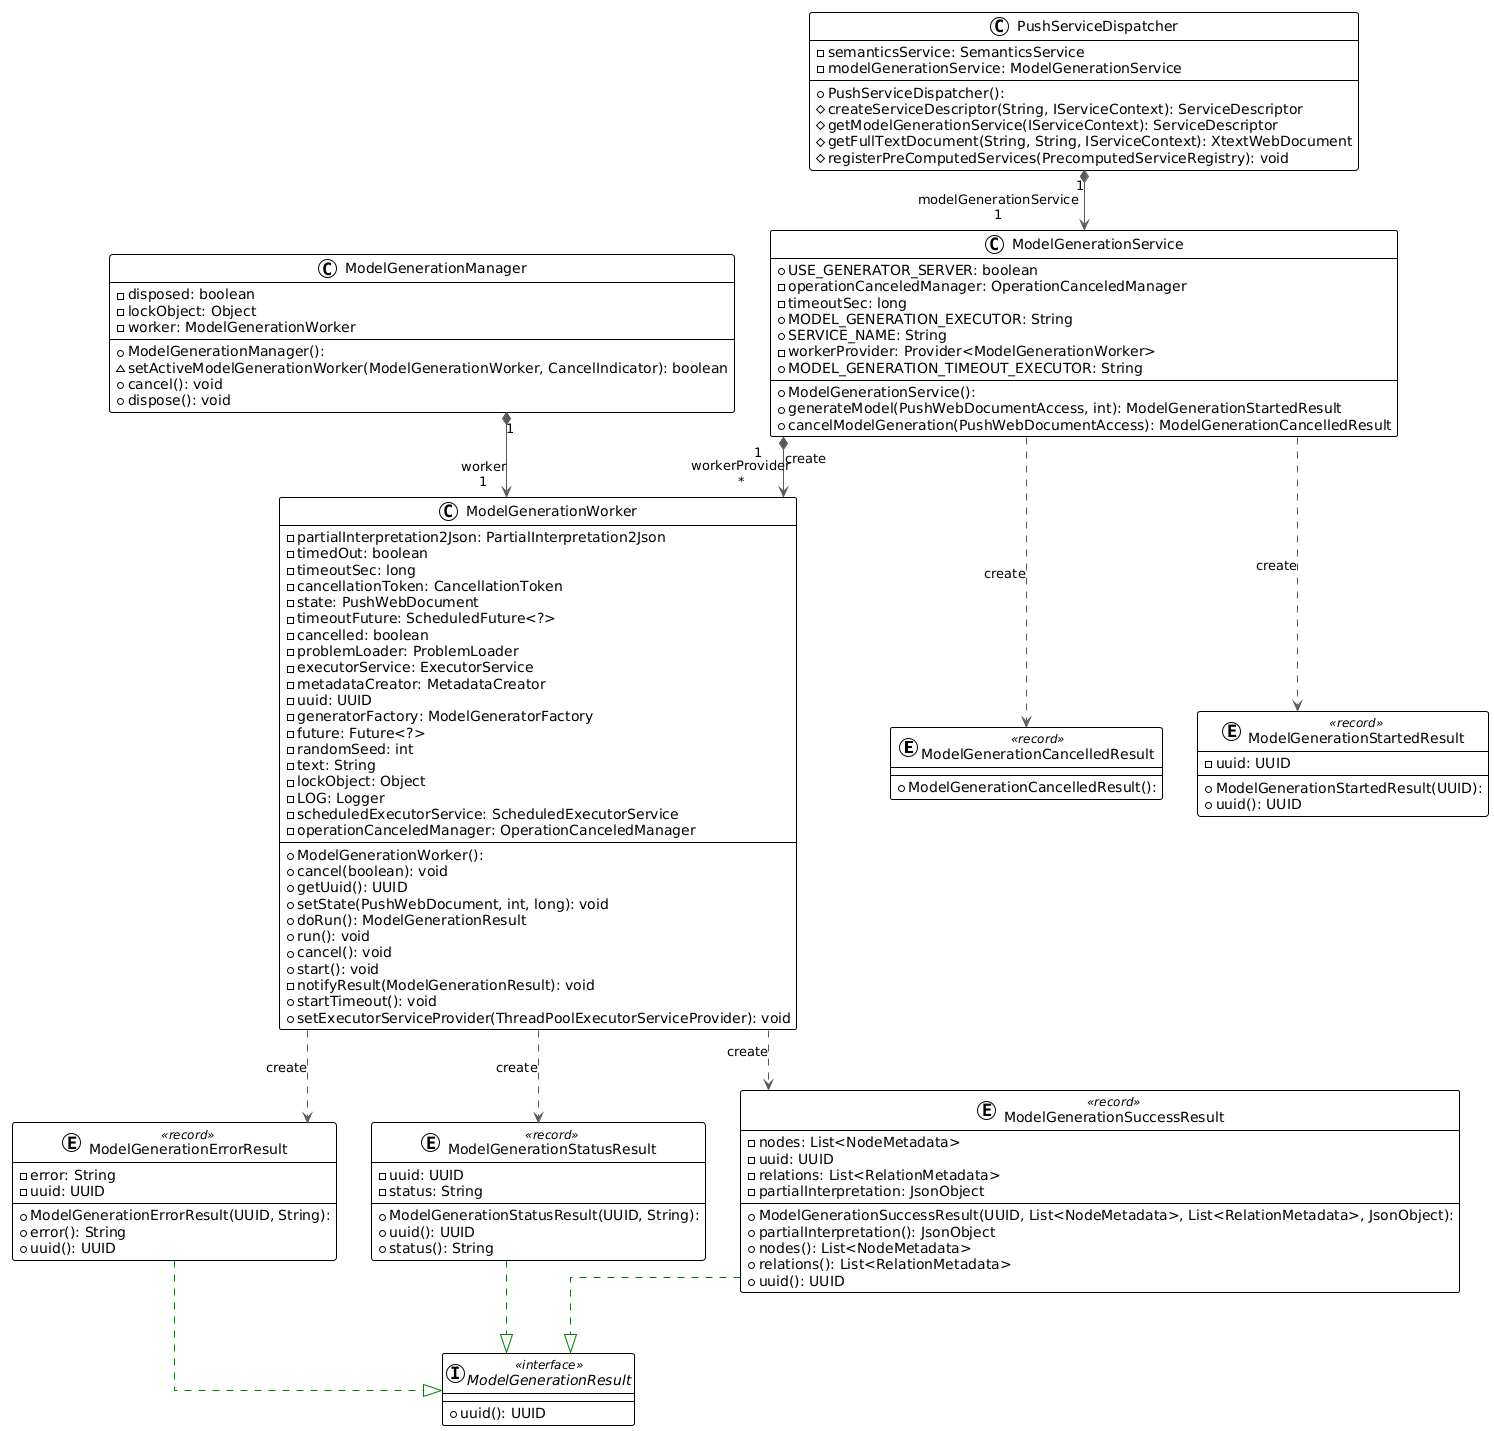
\includegraphics[scale=0.3]{include/imgs/backendUML.png}
		\caption{UML class diagram of the backend architecture}
		\label{backendstarteruml}
\end{figure}

%----------------------------------------------------------------------------
\clearpage\section{Generation Client}
%----------------------------------------------------------------------------
\begin{figure}[h!]
		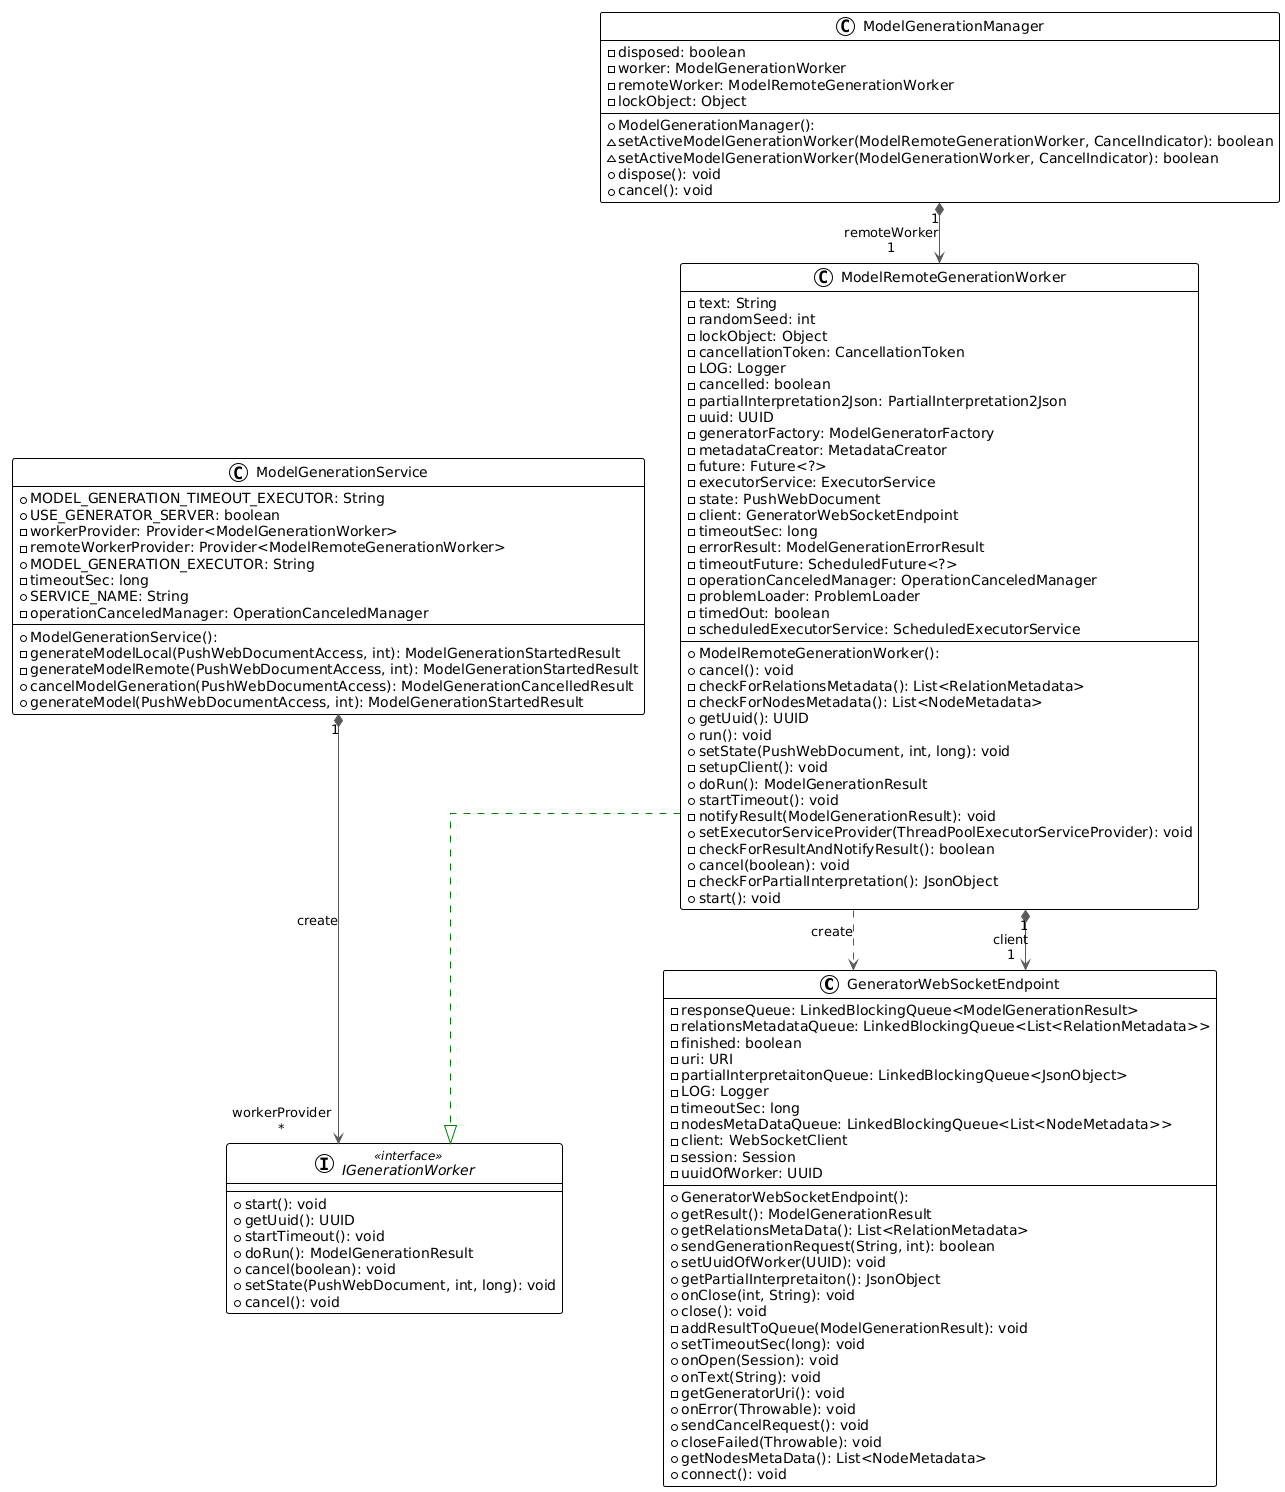
\includegraphics[scale=0.35]{include/imgs/generation_client_UML.png}
		\caption{UML class diagram of the generation client part of the backend}
		\label{backendclientuml}
\end{figure}

\clearpage\section{Generator Server}
%----------------------------------------------------------------------------
\begin{figure}[h!]
		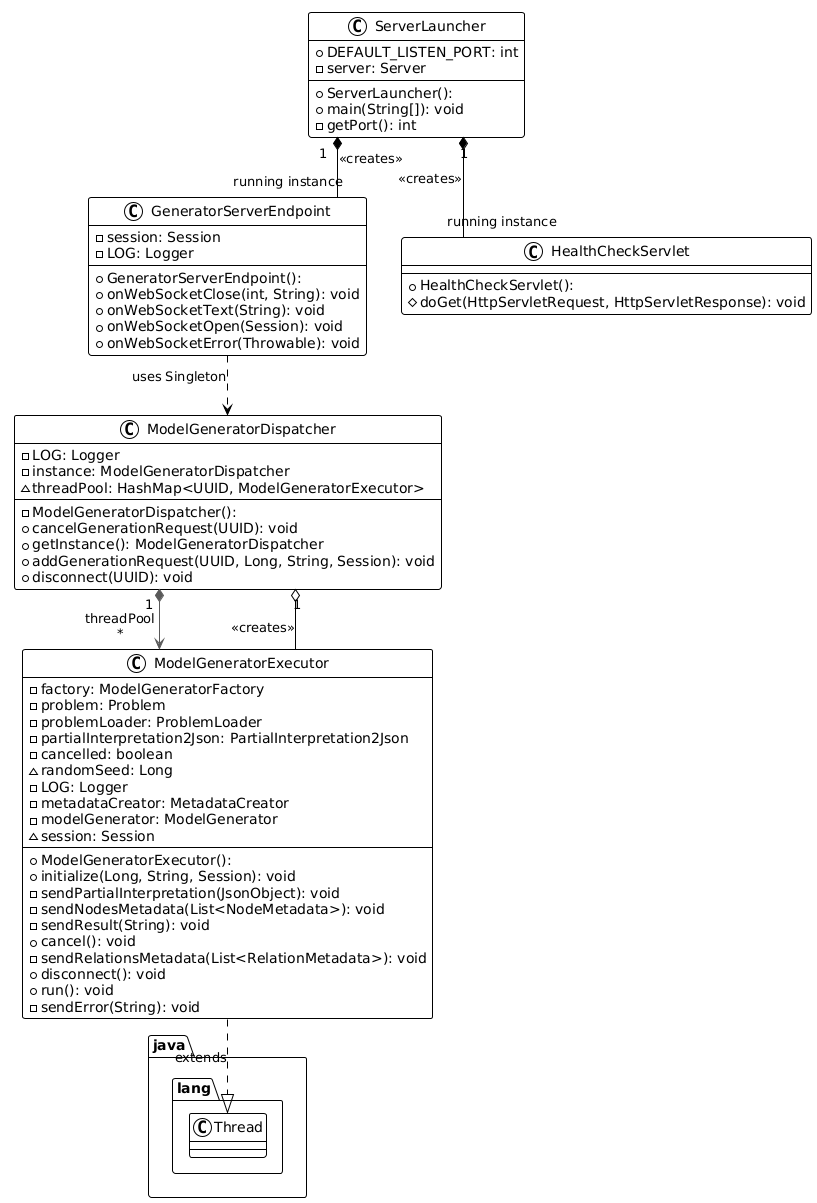
\includegraphics[scale=0.5]{include/imgs/generator_server_UML.png}
		\caption{UML class diagram of the generator server}
		\label{generatorserveruml}
\end{figure}

%\label{page:last}
\end{document}
